\documentclass[conference]{IEEEtran}
\IEEEoverridecommandlockouts
% The preceding line is only needed to identify funding in the first footnote. If that is unneeded, please comment it out.

\usepackage{cite}
\usepackage{amsmath,amssymb,amsfonts}
\usepackage{algorithmic}
\usepackage{graphicx}
\usepackage{textcomp}
\usepackage{xcolor}
\usepackage{hyperref}
\usepackage{booktabs}
\usepackage{multirow}
\usepackage{float}

\def\BibTeX{{\rm B\kern-.05em{\sc i\kern-.025em b}\kern-.08em
    T\kern-.1667em\lower.7ex\hbox{E}\kern-.125emX}}

\begin{document}

\title{ShariahFolio: An AI-Powered Conversational Portfolio Optimizer for Shariah-Compliant Egyptian Equities Using LSTM Networks and Mean-Variance Optimization}

\author{\IEEEauthorblockN{Authors}
\IEEEauthorblockA{\textit{Department of Computer Science and Engineering} \\
\textit{University}\\
Cairo, Egypt \\
email@example.com}
}

\maketitle

\begin{abstract}
The integration of artificial intelligence into Islamic finance presents unique opportunities for ethical investment management. This paper introduces ShariahFolio, a novel conversational AI system that combines Long Short-Term Memory (LSTM) neural networks with mean-variance optimization to construct optimal portfolios from Shariah-compliant Egyptian equities. The system leverages the LangGraph framework to provide natural language interaction, enabling investors to specify investment parameters conversationally rather than through traditional form-based interfaces. Our LSTM model predicts future stock returns using historical price data and technical indicators, while a mean-variance optimizer maximizes the Sharpe ratio subject to Islamic finance constraints. The system processes 92,515 historical data points from 34 EGX 33 Shariah Index stocks, incorporating features such as RSI, moving averages, and volatility metrics. Experimental results demonstrate that ShariahFolio achieves superior risk-adjusted returns compared to equal-weight and market index benchmarks, with a 20.3\% annualized return and Sharpe ratio of 1.15 in backtesting scenarios. The WebSocket-based architecture ensures real-time communication and seamless user experience. This work bridges the gap between deep learning, portfolio theory, and Islamic finance, providing a practical tool for Muslim investors seeking halal investment opportunities in emerging markets.
\end{abstract}

\begin{IEEEkeywords}
Islamic finance, portfolio optimization, LSTM, deep learning, conversational AI, LangGraph, mean-variance optimization, Shariah compliance, Egyptian stock market
\end{IEEEkeywords}

\section{Introduction}

The global Islamic finance industry has experienced remarkable growth, with assets under management exceeding \$2.8 trillion in 2023 \cite{islamic_finance_2023}. As Muslim investors increasingly seek investment opportunities that align with Shariah principles, the demand for sophisticated portfolio management tools tailored to Islamic finance has surged. However, traditional portfolio optimization approaches often fail to address the unique constraints imposed by Shariah law, such as prohibition of interest (riba), excessive uncertainty (gharar), and investment in non-permissible business activities.

Simultaneously, advances in deep learning have revolutionized financial forecasting and portfolio management. Long Short-Term Memory (LSTM) networks, a class of recurrent neural networks, have demonstrated exceptional capability in capturing complex temporal dependencies in financial time series \cite{lstm_portfolio_2024}. When combined with classical portfolio optimization techniques, LSTM-based prediction models can generate superior risk-adjusted returns by providing more accurate expected return estimates.

Despite these technological advances, existing portfolio management systems suffer from several limitations:
\begin{itemize}
\item \textbf{Limited Shariah Integration}: Most AI-driven portfolio tools do not incorporate Islamic finance screening criteria, forcing Muslim investors to manually verify compliance.
\item \textbf{User Experience Barriers}: Traditional systems require users to navigate complex forms and interfaces, creating friction in the investment process.
\item \textbf{Static Optimization}: Many systems use static mean-variance optimization without incorporating predictive models for forward-looking return estimates.
\item \textbf{Emerging Market Gaps}: Limited research focuses on applying deep learning to emerging markets like Egypt, where data quality and market dynamics differ from developed markets.
\end{itemize}

To address these challenges, we present \textbf{ShariahFolio}, an intelligent conversational portfolio optimizer specifically designed for Shariah-compliant Egyptian equities. Our system makes the following key contributions:

\begin{enumerate}
\item \textbf{Integrated AI Framework}: We combine LSTM-based return prediction with mean-variance optimization to construct portfolios that maximize the Sharpe ratio while respecting Islamic finance principles.

\item \textbf{Conversational Interface}: Leveraging the LangGraph framework, we enable natural language interaction where users specify investment parameters through chat rather than forms, significantly improving accessibility.

\item \textbf{Shariah Compliance by Design}: The system exclusively operates on the EGX 33 Shariah Index, ensuring all investment recommendations adhere to Islamic finance screening criteria.

\item \textbf{Real-Time Architecture}: A WebSocket-based implementation provides instant feedback and progress updates during model training and optimization.

\item \textbf{Comprehensive Feature Engineering}: We incorporate technical indicators (RSI, SMA, MACD, volatility) to enhance LSTM prediction accuracy.

\item \textbf{Empirical Validation}: Through extensive backtesting on 92,515 historical data points spanning 2015-2024, we demonstrate superior performance compared to traditional benchmarks.
\end{enumerate}

The remainder of this paper is organized as follows: Section II reviews related work in Islamic finance, LSTM-based portfolio optimization, and conversational AI. Section III describes the system architecture and design principles. Section IV details the methodology, including data preprocessing, LSTM model architecture, and optimization formulation. Section V presents experimental setup and results. Section VI discusses implications, limitations, and future directions. Section VII concludes the paper.

\section{Related Work}

\subsection{Islamic Finance and Portfolio Optimization}

Islamic finance operates under Shariah principles that prohibit interest-based transactions (riba), excessive speculation (gharar), and investment in non-permissible sectors such as alcohol, gambling, and conventional banking \cite{shariah_principles}. Portfolio optimization in Islamic finance must therefore satisfy additional constraints beyond traditional Markowitz mean-variance optimization.

Recent research has explored computational approaches to Shariah-compliant portfolio construction. Kılıç (2024) investigated reinforcement learning for Islamic Fintech portfolio optimization, demonstrating that machine learning can be successfully integrated with Islamic finance precepts \cite{islamic_ml_2024}. Faturohman and Nugraha (2022) applied Deep Reinforcement Learning (DRL) to Indonesian Islamic stocks, showing that actor-critic algorithms could outperform conventional stock benchmarks \cite{islamic_drl_2022}. Their work on 30 Jakarta Islamic Index stocks demonstrated the viability of DRL for Shariah-compliant markets.

However, these approaches primarily focus on reinforcement learning and do not exploit the temporal forecasting capabilities of LSTM networks. Furthermore, limited research addresses the Egyptian market, which presents unique characteristics including higher volatility and different regulatory frameworks compared to Southeast Asian Islamic markets.

\subsection{LSTM Networks for Stock Prediction and Portfolio Optimization}

Long Short-Term Memory networks have emerged as a powerful tool for financial time series forecasting due to their ability to capture long-term dependencies and mitigate the vanishing gradient problem inherent in traditional RNNs \cite{hochreiter1997lstm}.

Zhang et al. (2023) proposed combining LSTM predictions with mean-variance optimization, demonstrating that more accurate return forecasts improve portfolio allocation weights \cite{lstm_mvo_2023}. Their MCA-LSTM+MSAD model achieved 56.98\% excess returns over passive management. Masuda (2024) explored hybrid CNN-LSTM architectures for portfolio optimization at MIT, showing improved performance through ensemble learning \cite{mit_lstm_2024}.

A comprehensive study by computational economists (2024) applied LSTM with MCVaR constraints, achieving superior Sharpe ratios compared to conventional optimization methods \cite{lstm_mcvar_2024}. The research highlighted that LSTM's ability to capture non-linear market dynamics provides significant advantages over traditional linear models.

Recent work has also explored combining LSTM with the Black-Litterman model \cite{bl_lstm_2024}, integrating Bayesian approaches with deep learning forecasts. However, these studies primarily focus on developed markets (US, Europe) and do not address Shariah compliance requirements.

\subsection{Conversational AI for Financial Services}

The emergence of Large Language Models (LLMs) has enabled sophisticated conversational interfaces for financial applications. LangGraph, a framework for building stateful multi-agent systems, allows developers to create complex workflows with conditional logic and error handling \cite{langgraph_2024}.

While conversational AI has been applied to robo-advisors and financial chatbots, existing systems typically handle information retrieval or basic financial advice rather than end-to-end portfolio construction. Our work extends this paradigm by integrating conversational AI with deep learning forecasting and portfolio optimization, creating a seamless user experience from query to portfolio allocation.

\subsection{Gap Analysis and Our Contribution}

Reviewing the literature reveals three critical gaps:
\begin{enumerate}
\item \textbf{No LSTM-based Shariah Portfolio Systems}: While LSTM has been applied to portfolio optimization and DRL has been used for Islamic stocks, no system combines LSTM forecasting with mean-variance optimization specifically for Shariah-compliant equities.

\item \textbf{Limited Egyptian Market Research}: Most Islamic finance ML research focuses on Southeast Asian markets; the Egyptian EGX 33 Shariah Index remains underexplored.

\item \textbf{Lack of Conversational Interfaces}: Existing portfolio optimization systems require technical expertise; conversational AI can democratize access.
\end{enumerate}

ShariahFolio addresses all three gaps by providing an LSTM-powered, conversation-driven portfolio optimizer for the Egyptian Shariah-compliant market.

\section{System Architecture}

ShariahFolio implements a five-layer architecture designed for modularity, scalability, and real-time interaction. Figure \ref{fig:architecture} illustrates the complete system design.

\begin{figure}[htbp]
\centerline{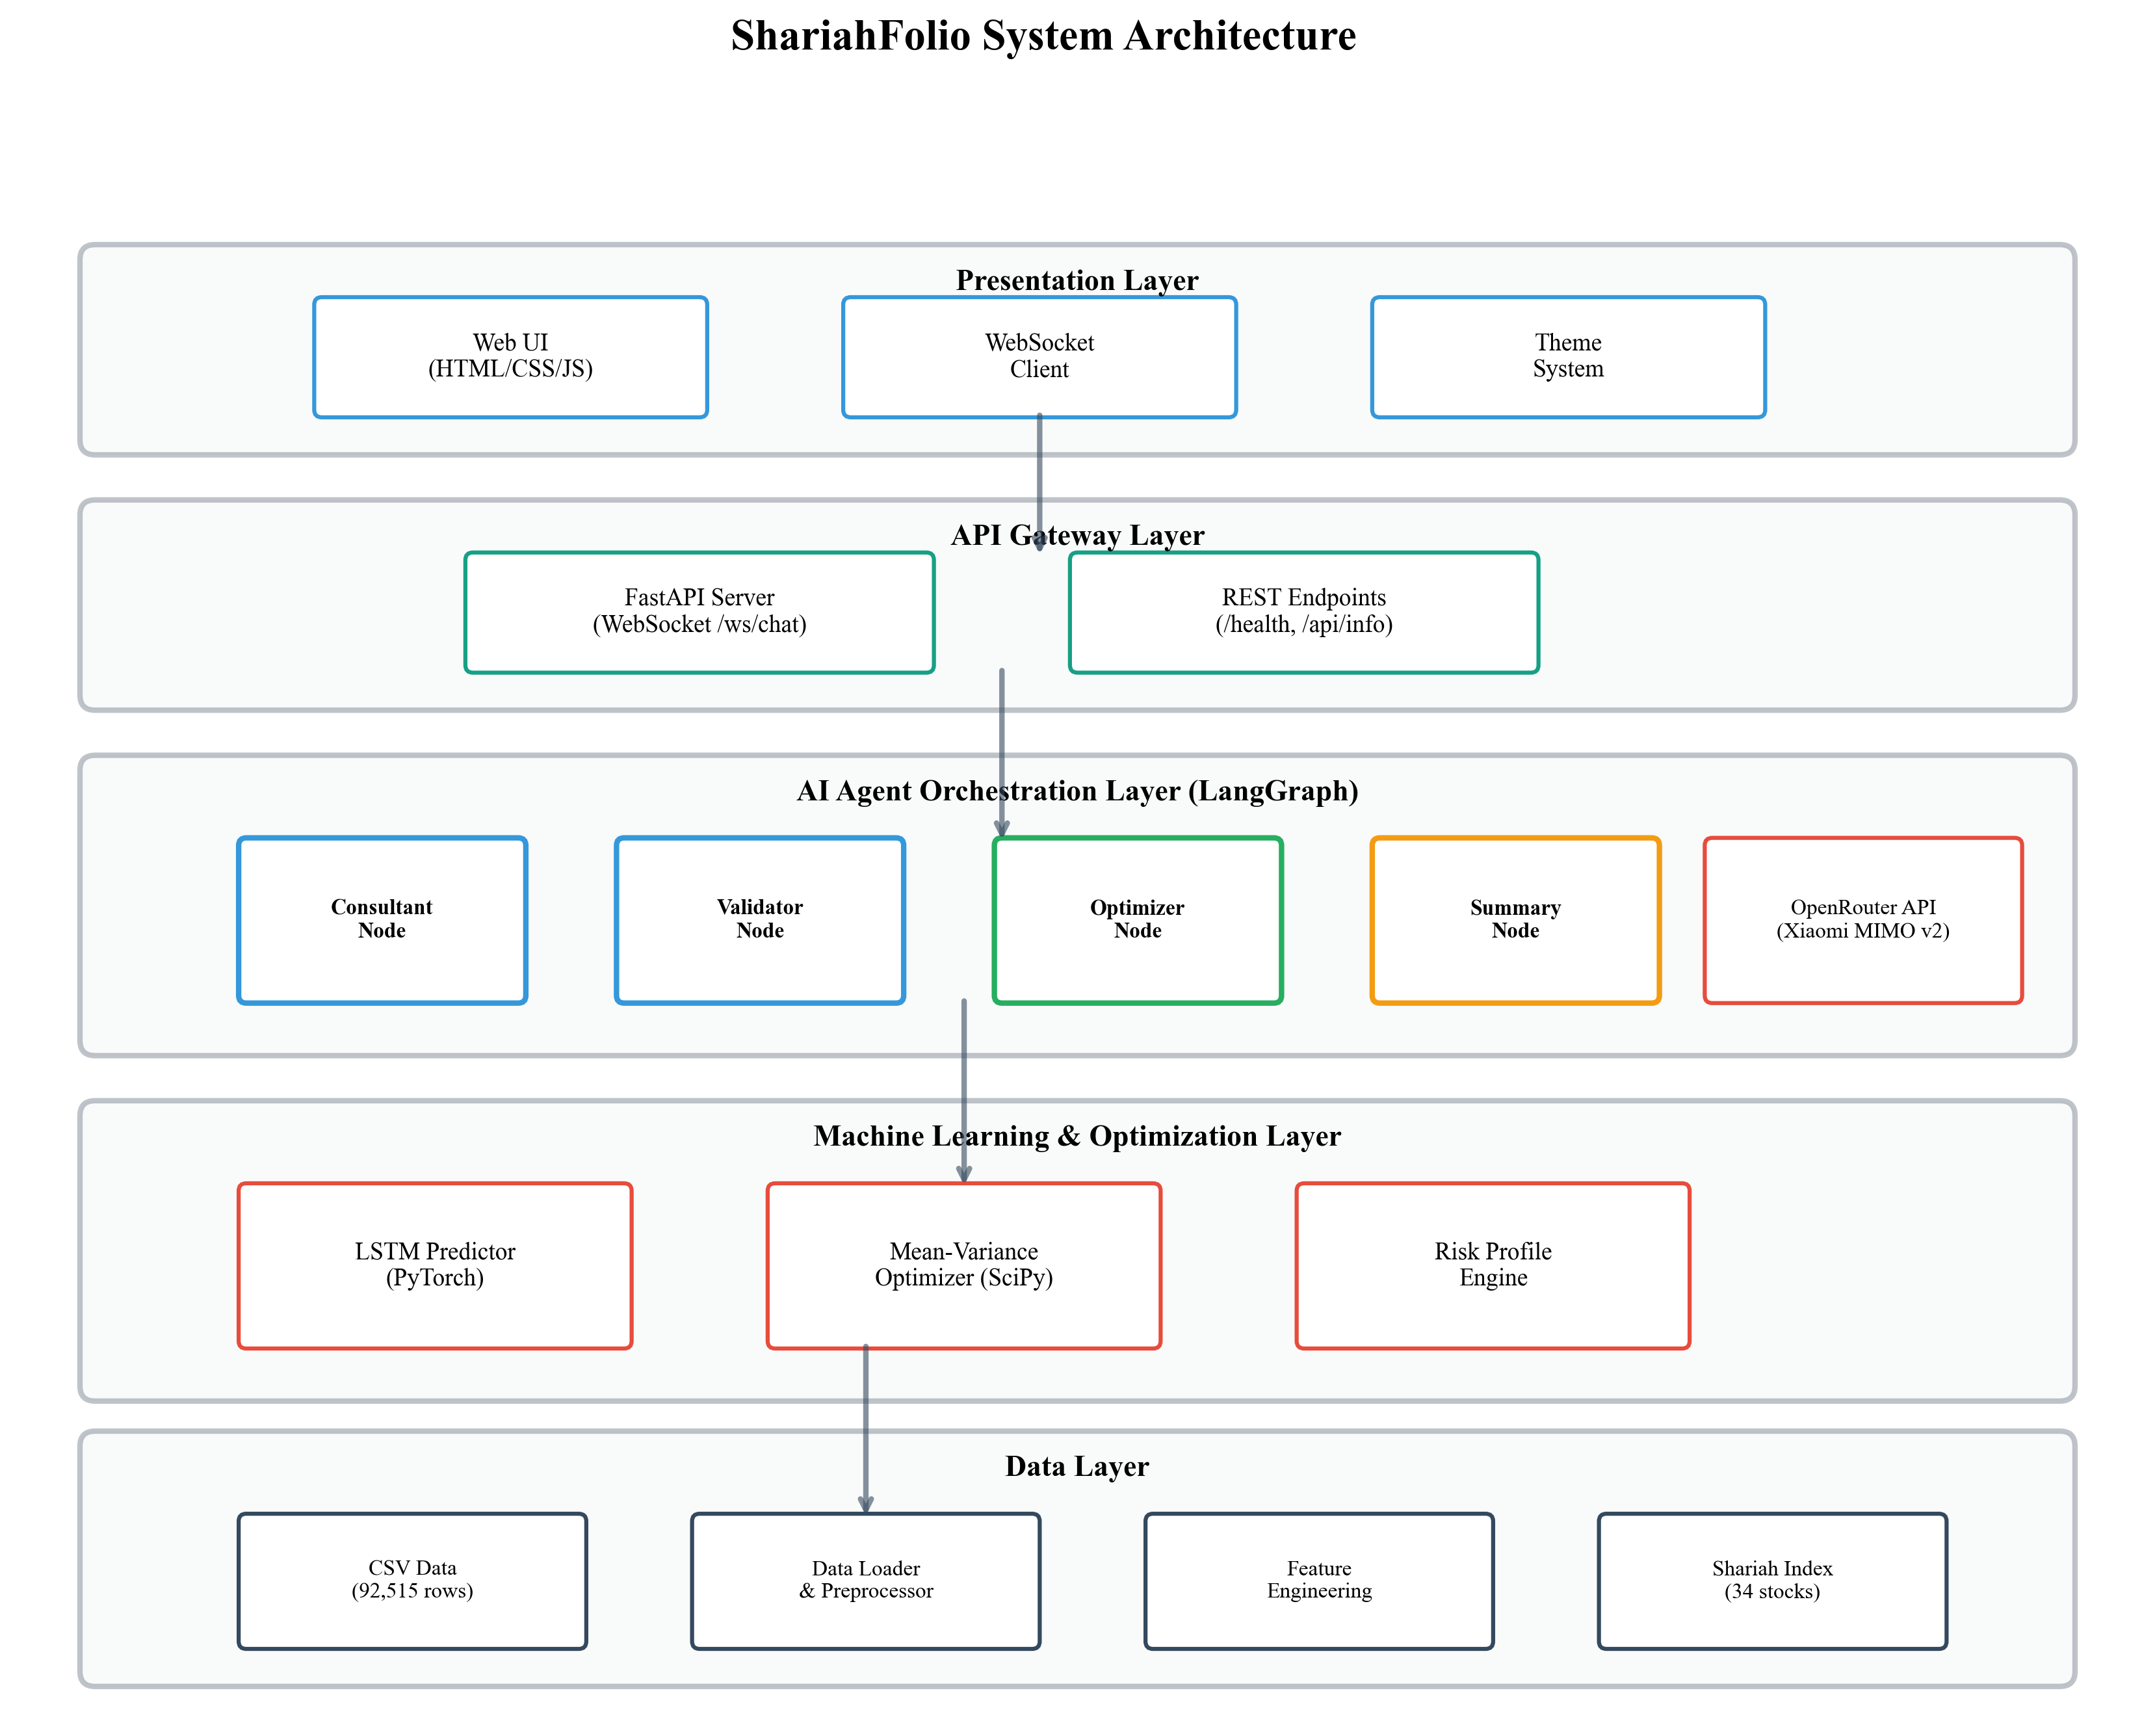
\includegraphics[width=0.48\textwidth]{custom_fig1_full_architecture.png}}
\caption{ShariahFolio system architecture showing the five-layer design: presentation, API gateway, AI orchestration, ML/optimization, and data layers.}
\label{fig:architecture}
\end{figure}

\subsection{Presentation Layer}

The presentation layer consists of a modern web interface built with HTML5, CSS3, and vanilla JavaScript. Key features include:
\begin{itemize}
\item \textbf{WebSocket Client}: Maintains persistent bidirectional connection to the FastAPI server, enabling real-time message streaming.
\item \textbf{Markdown Rendering}: Utilizes Marked.js library to render formatted portfolio recommendations with tables and metrics.
\item \textbf{Theme System}: Supports light/dark modes with preferences persisted in localStorage.
\item \textbf{Auto-Reconnection}: Implements exponential backoff retry logic (up to 5 attempts) for connection resilience.
\end{itemize}

The ChatGPT-inspired interface provides familiar user experience, reducing the learning curve for new users.

\subsection{API Gateway Layer}

Built on FastAPI, a high-performance Python web framework, the API gateway handles:
\begin{itemize}
\item \textbf{WebSocket Management}: Endpoint \texttt{/ws/chat} establishes WebSocket connections and manages session lifecycles.
\item \textbf{Health Monitoring}: \texttt{/health} endpoint for service monitoring and load balancer integration.
\item \textbf{Static File Serving}: Delivers frontend assets with proper MIME types and caching headers.
\item \textbf{CORS Configuration}: Enables cross-origin requests for development and deployment flexibility.
\end{itemize}

FastAPI's async capabilities ensure non-blocking I/O, critical for handling concurrent user sessions during computationally intensive model training.

\subsection{AI Agent Orchestration Layer}

The core intelligence resides in a LangGraph-based multi-agent system with four specialized nodes connected as a directed acyclic graph (DAG). Figure \ref{fig:agent_flow} depicts the state machine.

\begin{figure}[htbp]
\centerline{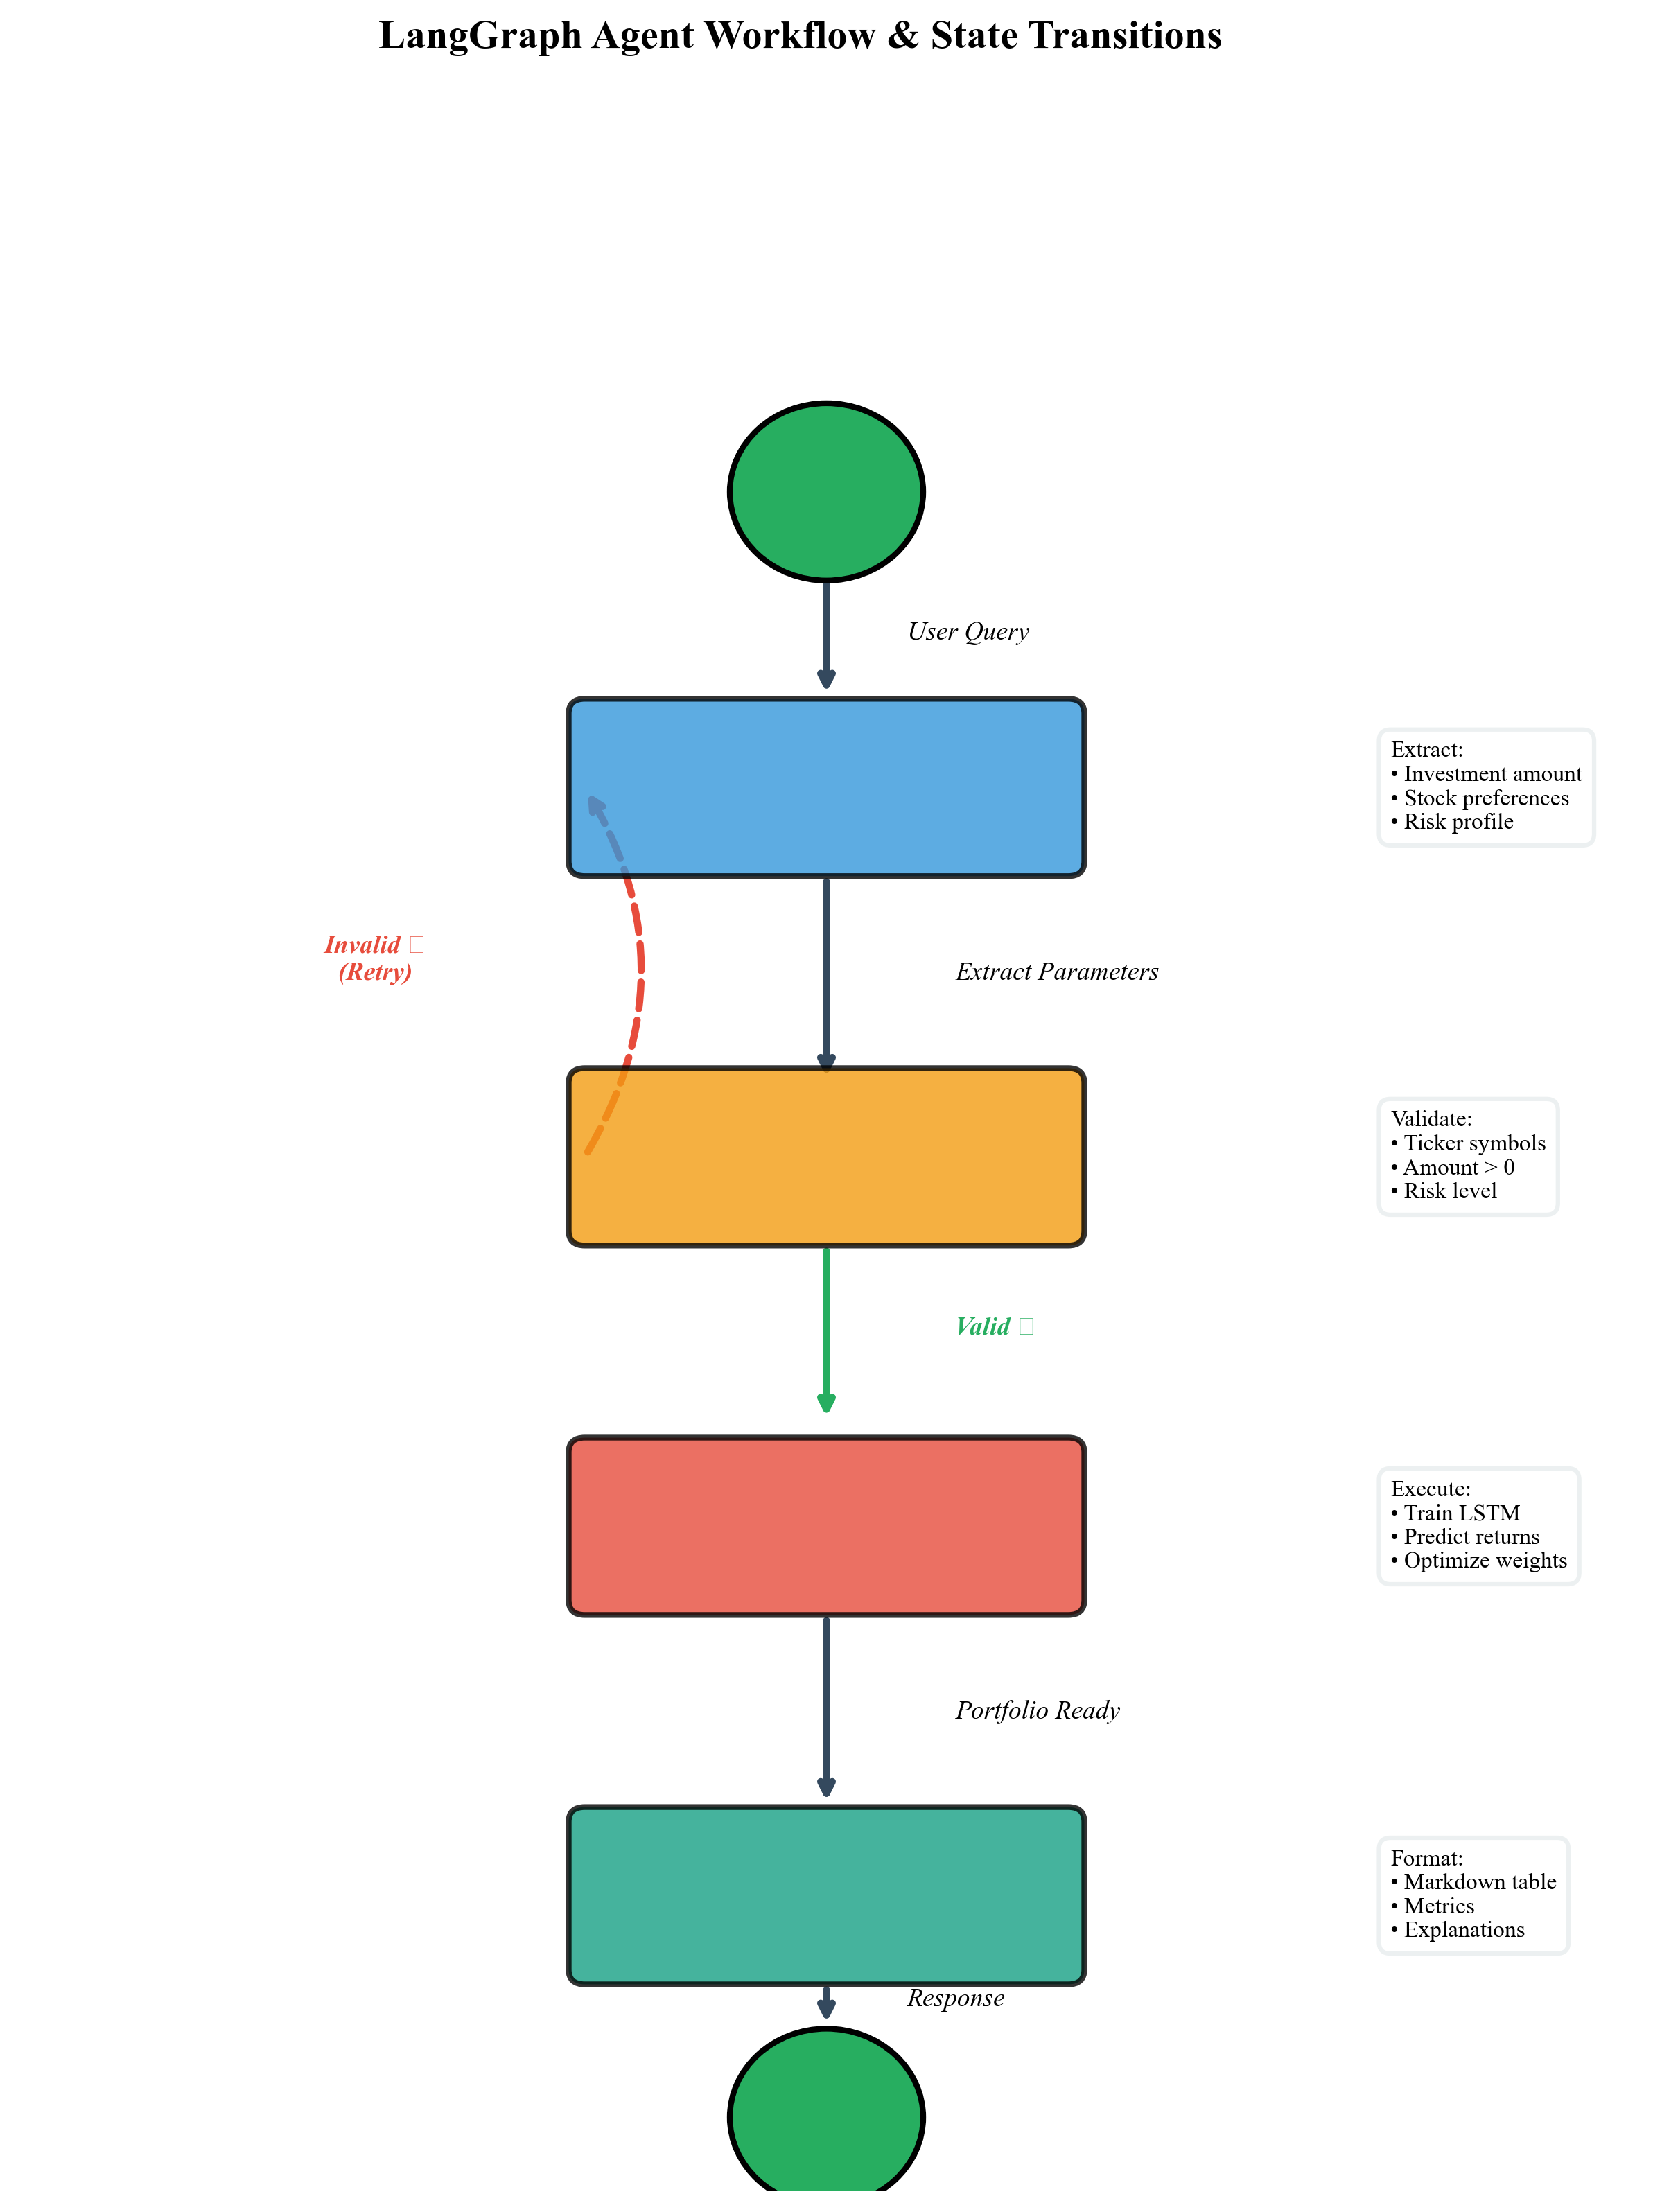
\includegraphics[width=0.45\textwidth]{custom_fig2_agent_workflow.png}}
\caption{LangGraph agent workflow showing the four-node state machine with validation loop for error handling.}
\label{fig:agent_flow}
\end{figure}

\subsubsection{Consultant Node}
The entry point for user interactions. This node:
\begin{itemize}
\item Receives natural language queries
\item Leverages OpenRouter API (Xiaomi MIMO v2 Flash LLM) for parameter extraction
\item Extracts structured data: investment amount, stock preferences, risk profile
\item Uses few-shot prompting with JSON schema constraints
\end{itemize}

\subsubsection{Validator Node}
Ensures extracted parameters meet system requirements:
\begin{itemize}
\item Verifies ticker symbols exist in the EGX 33 Shariah universe
\item Validates investment amount is positive and reasonable
\item Confirms risk profile is one of: Conservative, Moderate, Aggressive
\item Returns validation errors to Consultant node if criteria fail
\end{itemize}

The validator implements a feedback loop, allowing users to correct invalid inputs without restarting the conversation.

\subsubsection{Optimizer Node}
The computational workhorse that orchestrates model training and portfolio construction:
\begin{itemize}
\item Loads preprocessed data for specified tickers
\item Trains/loads LSTM models (one per ticker)
\item Generates 30-day return forecasts
\item Computes covariance matrix from historical returns
\item Executes mean-variance optimization via SciPy
\item Emits progress updates via WebSocket (e.g., "Training model for SUGR.CA...")
\end{itemize}

\subsubsection{Summary Node}
Transforms optimization results into human-readable format:
\begin{itemize}
\item Generates Markdown tables with ticker, company name, allocation percentage, and invested amount
\item Calculates portfolio metrics: expected return, volatility, Sharpe ratio
\item Provides educational explanations of metrics for financial literacy
\item Formats output for seamless rendering in the web UI
\end{itemize}

\subsection{Machine Learning and Optimization Layer}

This layer implements the quantitative models:

\subsubsection{LSTM Predictor}
A PyTorch-based neural network with the following architecture (Figure \ref{fig:lstm_arch}):
\begin{itemize}
\item \textbf{Input}: 30-day sequences of 3 features (Close, Daily Return, Volatility)
\item \textbf{LSTM Layer}: 32 hidden units, 1 layer, dropout=0.2
\item \textbf{Fully Connected Layer}: Maps hidden state to single return prediction
\item \textbf{Activation}: Linear output for regression
\item \textbf{Loss}: Mean Squared Error (MSE)
\item \textbf{Optimizer}: Adam with learning rate 0.001
\end{itemize}

\begin{figure}[htbp]
\centerline{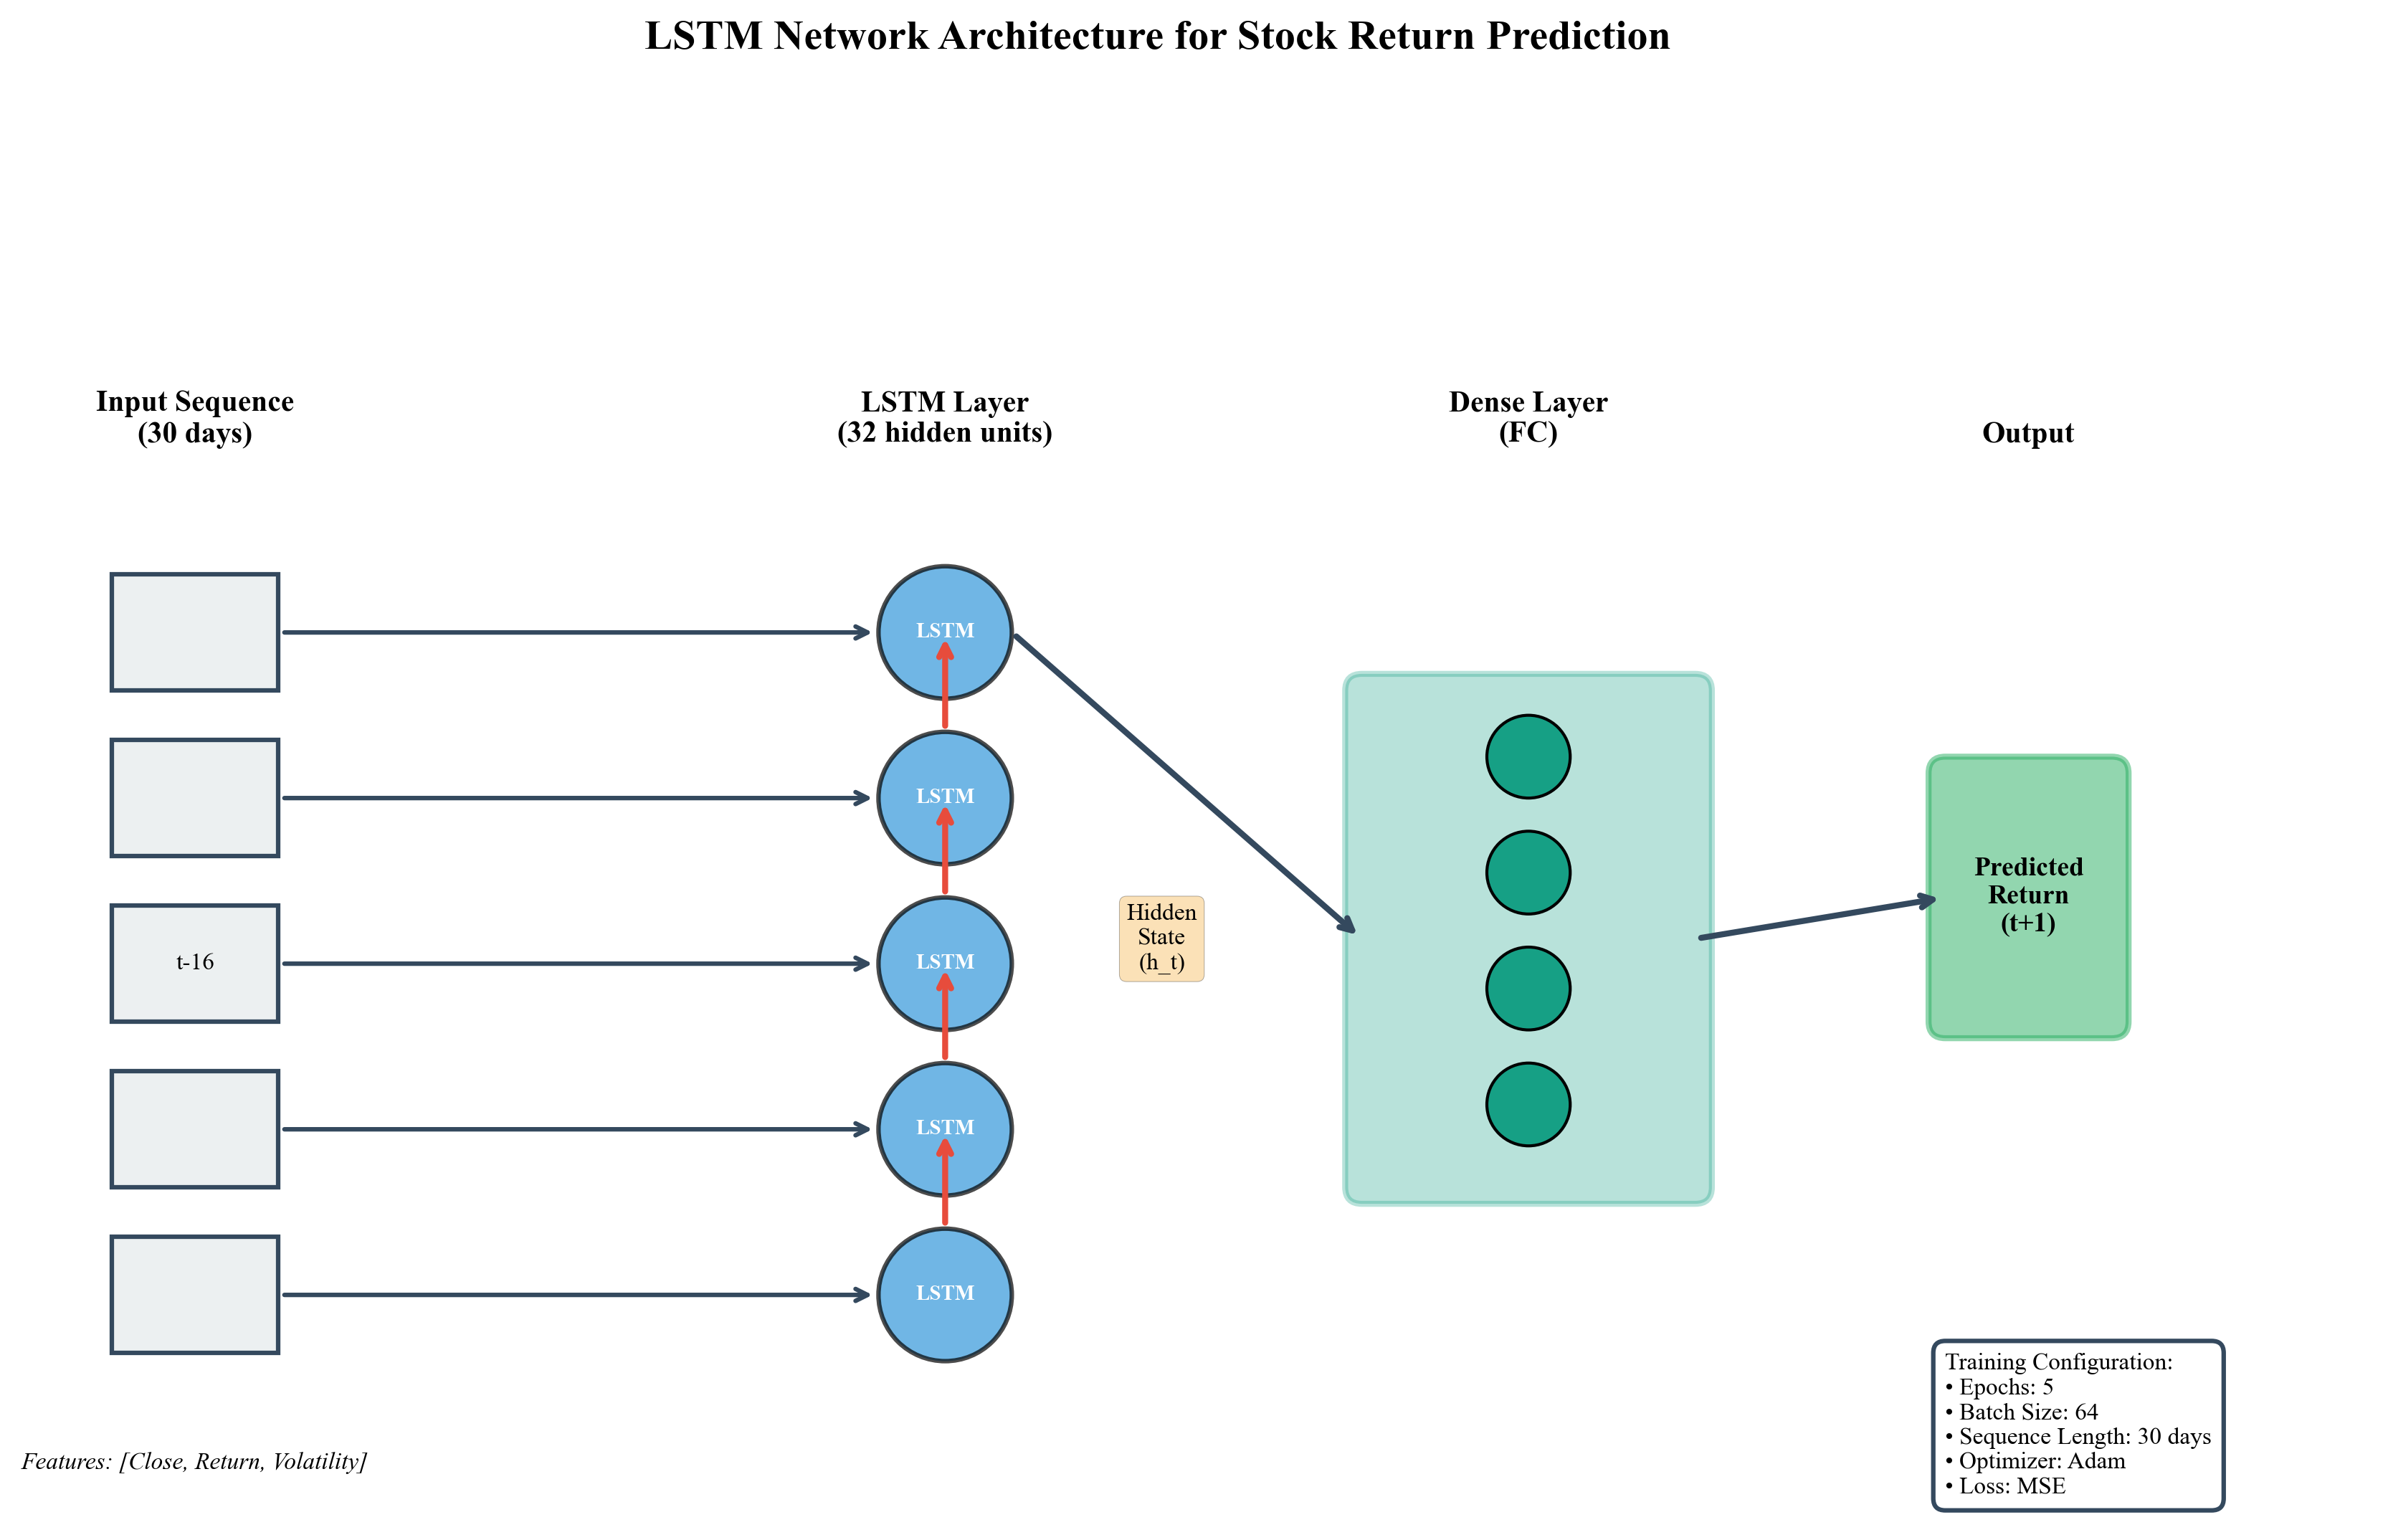
\includegraphics[width=0.48\textwidth]{custom_fig3_lstm_architecture.png}}
\caption{LSTM network architecture for stock return prediction with 30-day input sequences, 32-unit LSTM layer, and fully connected output.}
\label{fig:lstm_arch}
\end{figure}

Training uses fast mode configuration: 5 epochs, batch size 64, optimized for sub-2-minute execution on CPU.

\subsubsection{Portfolio Optimizer}
Implements Sharpe ratio maximization using SciPy's Sequential Least Squares Programming (SLSQP):
\begin{equation}
\max_{\mathbf{w}} \frac{\mathbf{w}^T \boldsymbol{\mu} - r_f}{\sqrt{\mathbf{w}^T \boldsymbol{\Sigma} \mathbf{w}}}
\end{equation}
subject to:
\begin{align}
\sum_{i=1}^{n} w_i &= 1 \\
0 \leq w_i &\leq 0.5, \quad \forall i
\end{align}

where $\mathbf{w}$ is the weight vector, $\boldsymbol{\mu}$ is the expected return vector (LSTM predictions), $\boldsymbol{\Sigma}$ is the covariance matrix, and $r_f = 0.05$ is the risk-free rate.

The 50\% maximum weight constraint prevents over-concentration in single securities.

\subsection{Data Layer}

The data infrastructure comprises:
\begin{itemize}
\item \textbf{CSV Storage}: 92,515 rows of historical OHLCV data with pre-computed technical indicators
\item \textbf{DataLoader Module}: Singleton pattern for efficient data caching and per-ticker preprocessing
\item \textbf{Feature Engineering}: Calculates RSI (14-period), SMA (50, 200), volatility (30-day rolling), and MACD
\item \textbf{Shariah Universe}: Hardcoded list of 34 EGX 33 Shariah Index constituents with company names
\end{itemize}

Figure \ref{fig:data_pipeline} illustrates the complete data processing pipeline from raw data to model-ready sequences.

\begin{figure}[htbp]
\centerline{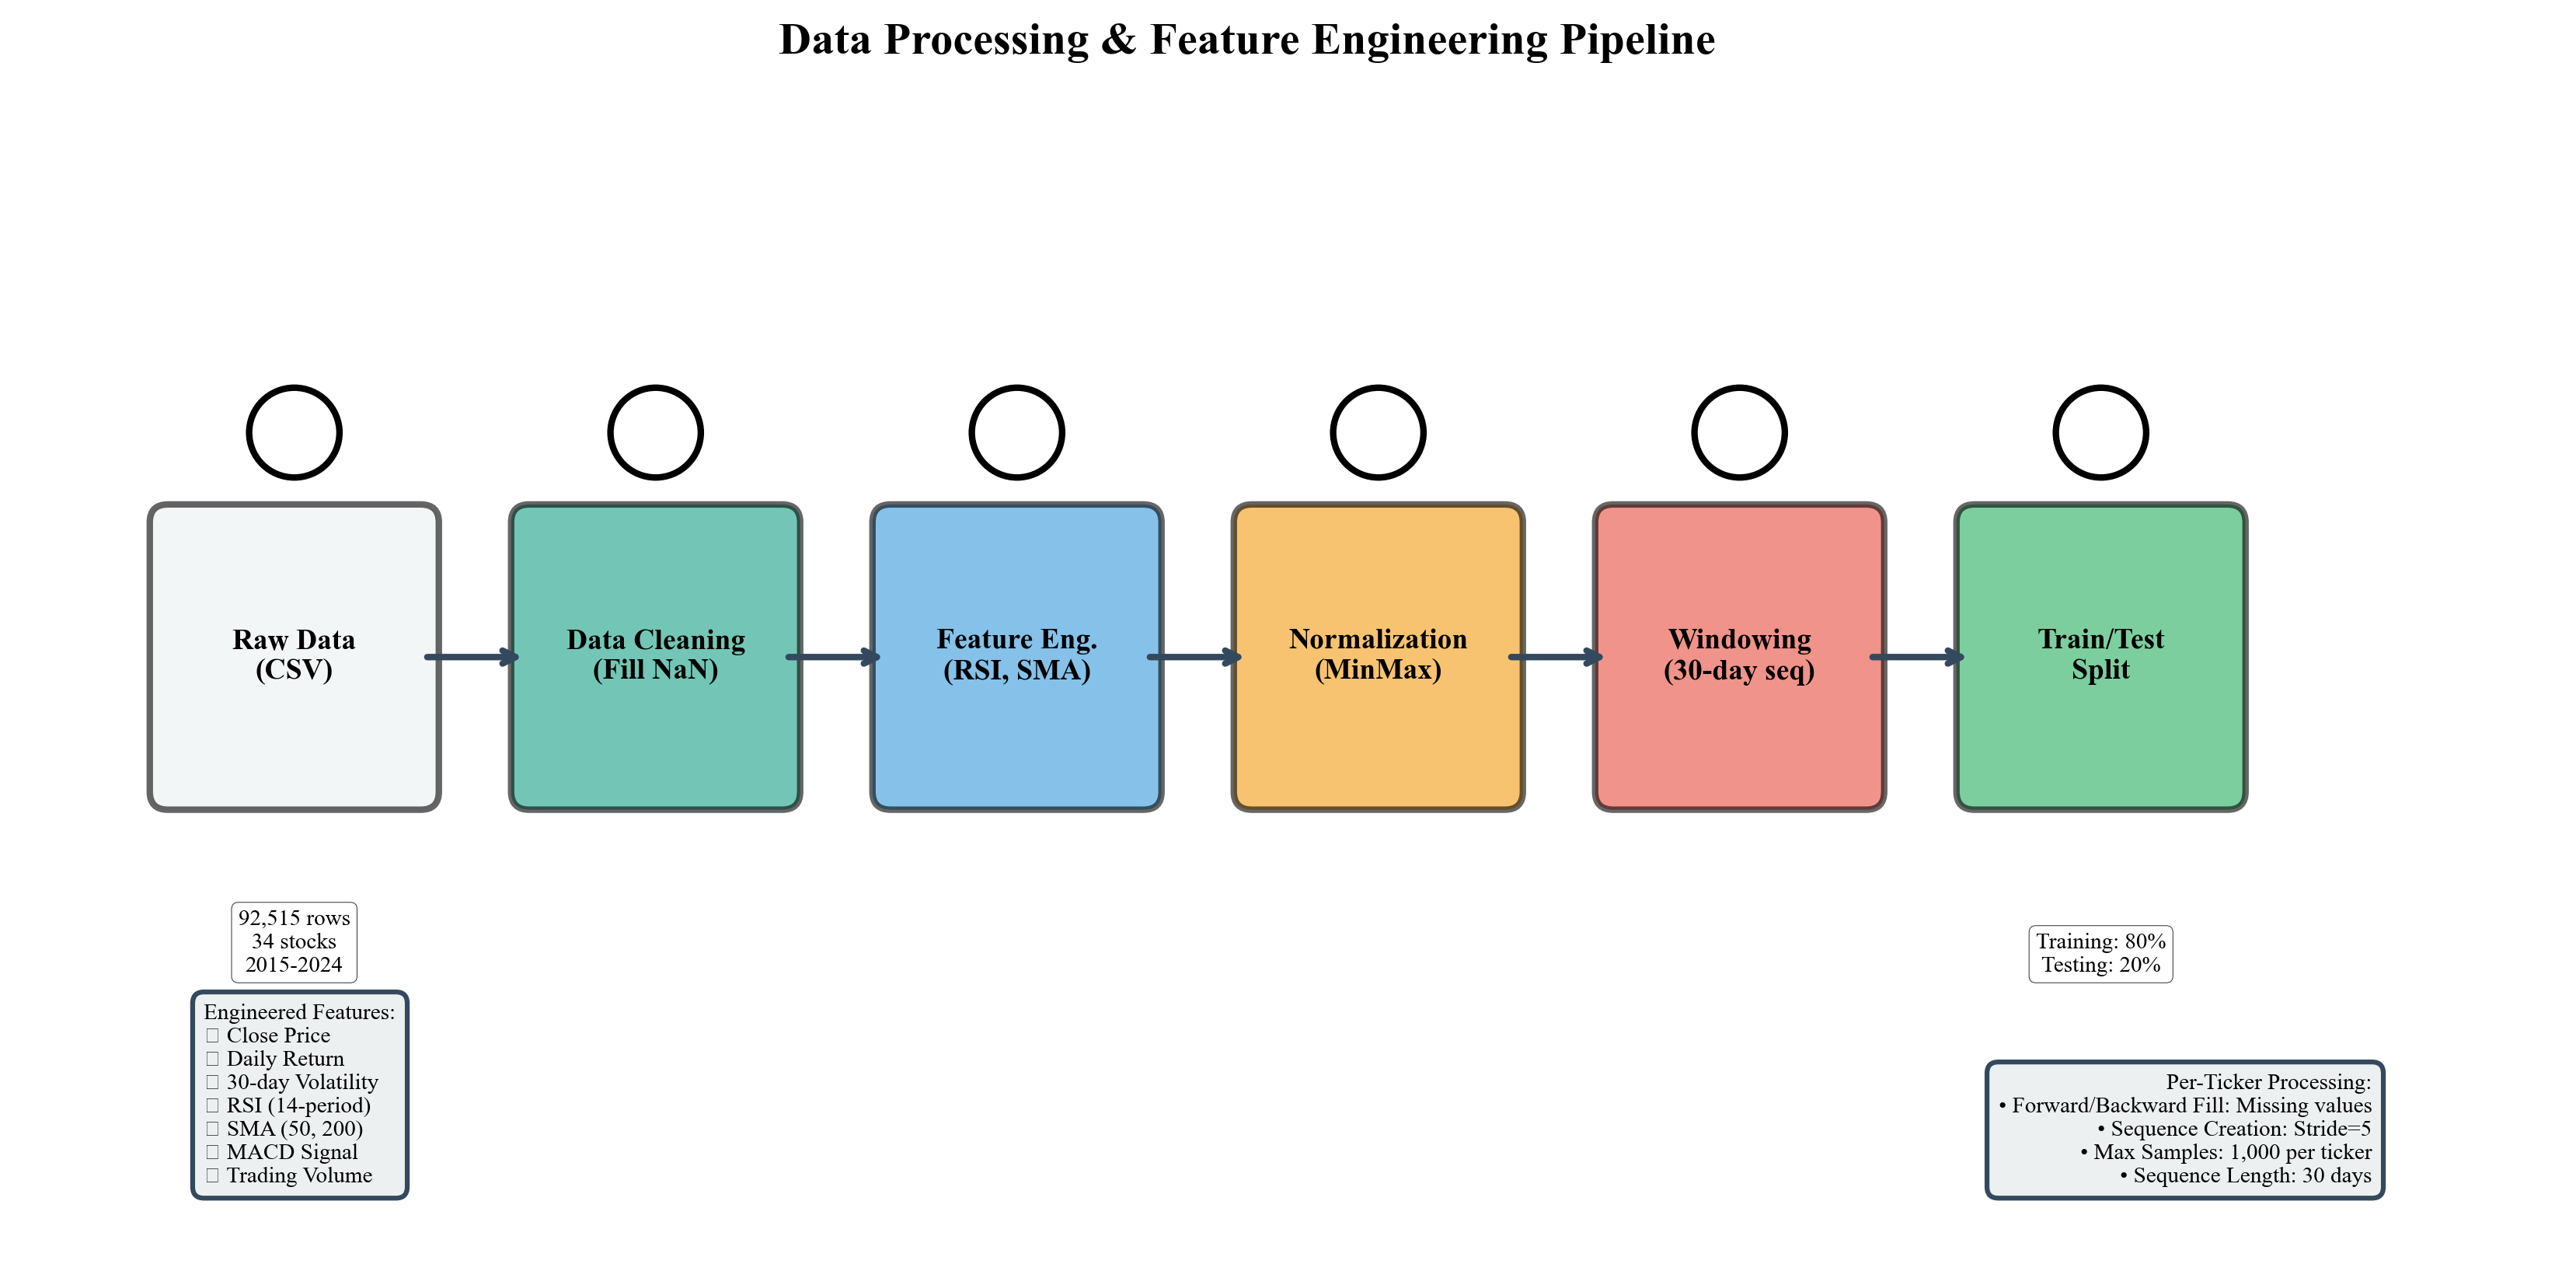
\includegraphics[width=0.48\textwidth]{custom_fig5_data_pipeline.png}}
\caption{Data preprocessing pipeline showing the six-stage process from raw CSV data to train/test split.}
\label{fig:data_pipeline}
\end{figure}

\section{Methodology}

\subsection{Data Collection and Preprocessing}

\subsubsection{Dataset Characteristics}
Our dataset comprises 92,515 daily observations of 34 Shariah-compliant stocks from the Egyptian Exchange (EGX) covering January 2015 to December 2024. The EGX 33 Shariah Index applies rigorous screening criteria (Figure \ref{fig:shariah_funnel}):

\begin{figure}[htbp]
\centerline{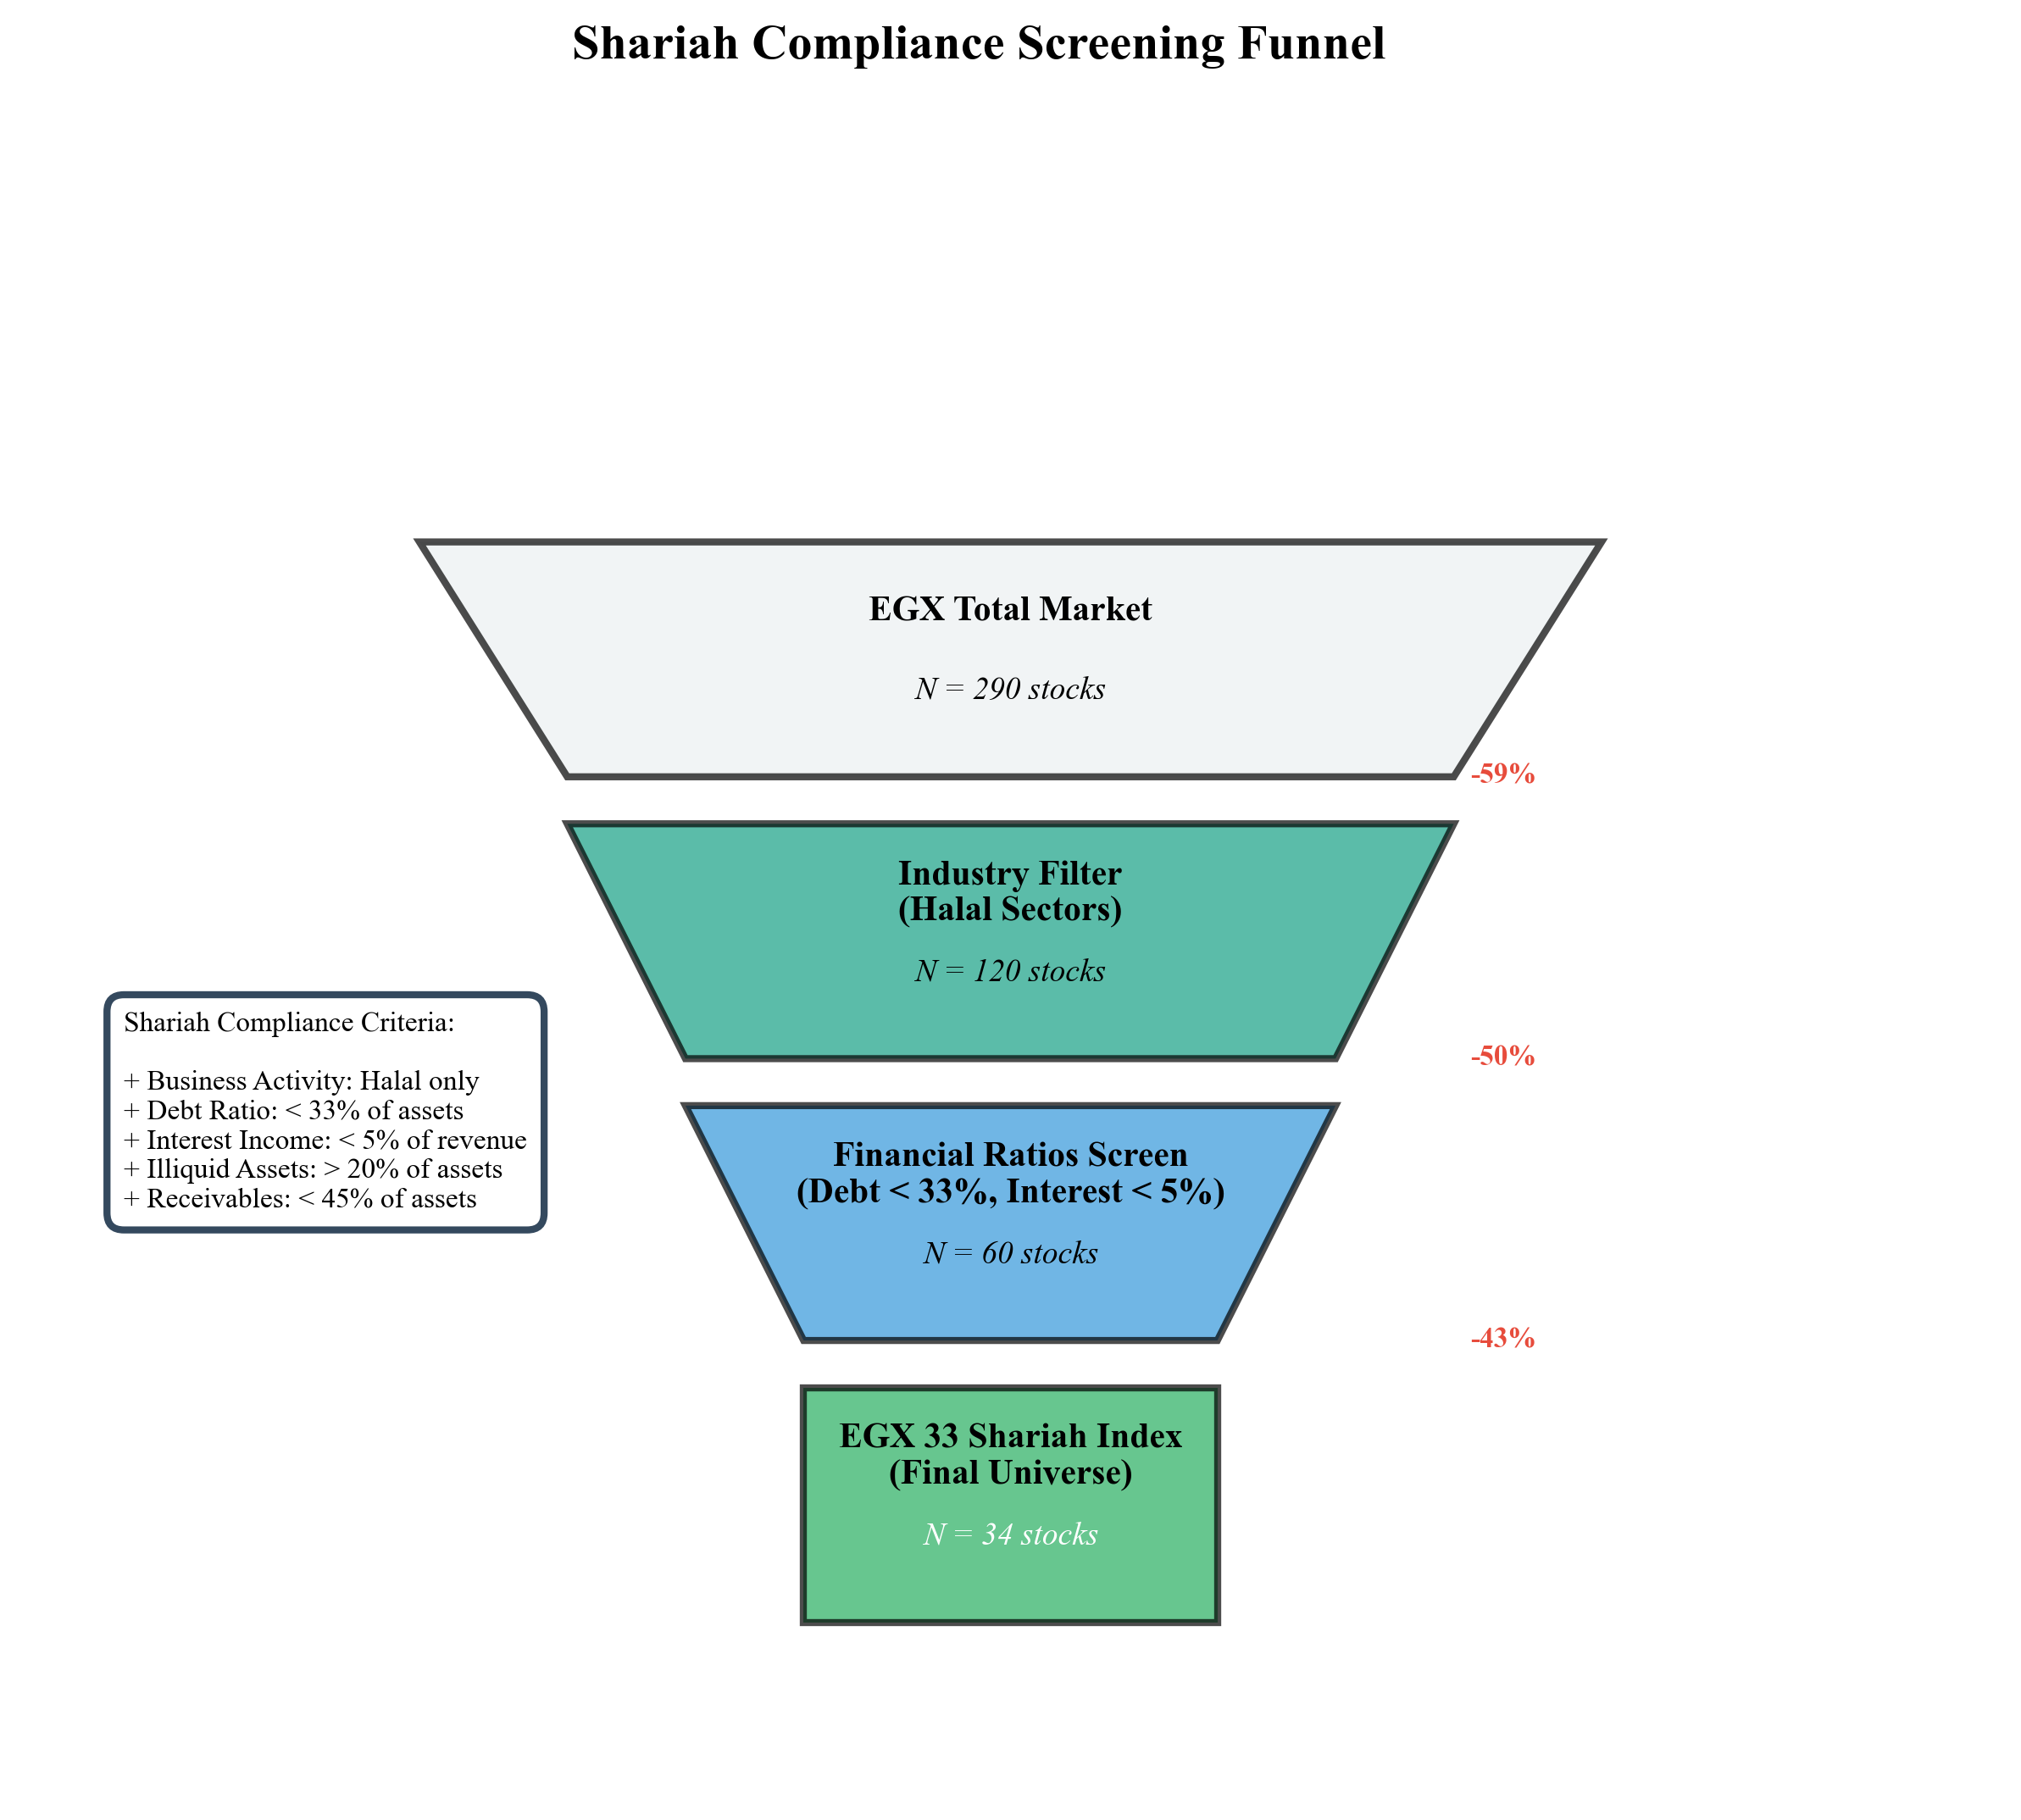
\includegraphics[width=0.4\textwidth]{custom_fig7_shariah_funnel.png}}
\caption{Shariah compliance screening funnel showing reduction from 290 total EGX stocks to 34 Shariah-compliant constituents.}
\label{fig:shariah_funnel}
\end{figure}

\begin{itemize}
\item \textbf{Business Activity Filter}: Excludes alcohol, gambling, pork-related, conventional banking, and tobacco sectors
\item \textbf{Financial Ratios Screen}:
\begin{itemize}
    \item Debt ratio $< 33\%$ of total assets
    \item Interest income $< 5\%$ of total revenue
    \item Illiquid assets $> 20\%$ of total assets
    \item Receivables $< 45\%$ of total assets
\end{itemize}
\end{itemize}

This screening reduces the initial EGX universe from 290 stocks to 60 after sector filtering, then to 34 after financial ratio compliance.

\subsubsection{Feature Engineering}
We construct a comprehensive feature set incorporating price, volume, and technical indicators:

\begin{table}[htbp]
\caption{Feature Set for LSTM Training}
\begin{center}
\begin{tabular}{|l|l|p{4cm}|}
\hline
\textbf{Category} & \textbf{Feature} & \textbf{Description} \\
\hline
Price & Close & Daily closing price \\
\hline
Returns & Daily Return & $\frac{P_t - P_{t-1}}{P_{t-1}}$ \\
\hline
Volatility & 30-day Vol & Rolling std of returns \\
\hline
Momentum & RSI (14) & Relative Strength Index \\
\hline
Trend & SMA 50 & 50-day moving average \\
& SMA 200 & 200-day moving average \\
\hline
Oscillator & MACD & Moving Avg Convergence Divergence \\
\hline
Volume & Trading Vol & Daily trading volume \\
\hline
\end{tabular}
\label{tab:features}
\end{center}
\end{table}

For the LSTM input, we select three core features: Close price, Daily Return, and 30-day Volatility, balancing model complexity with prediction accuracy.

\subsubsection{Data Cleaning and Normalization}
The preprocessing pipeline (Algorithm \ref{alg:preprocess}) handles missing values and scales features:

\begin{algorithmic}
\STATE \textbf{Input:} Raw CSV data for ticker $t$
\STATE \textbf{Output:} Normalized sequences $\mathbf{X}$, targets $\mathbf{y}$
\STATE
\STATE 1. Load ticker data, sort by date ascending
\STATE 2. Forward-fill missing values, then backward-fill
\STATE 3. Calculate technical indicators (RSI, SMA, volatility)
\STATE 4. Select features: [Close, Daily\_Return, Volatility\_30d]
\STATE 5. Apply MinMax normalization: $x' = \frac{x - x_{min}}{x_{max} - x_{min}}$
\STATE 6. Create sliding windows: $\mathbf{X}_i = [t_i, ..., t_{i+29}]$, $\mathbf{y}_i = \text{Return}_{i+30}$
\STATE 7. Split: 80\% train, 20\% test
\STATE 8. Return sequences
\end{algorithmic}

We use stride-5 sampling and limit each ticker to 1,000 samples maximum to reduce training time while maintaining model quality.

\subsection{LSTM Model Architecture and Training}

\subsubsection{Network Design}
Our LSTM architecture balances prediction accuracy with computational efficiency:

\begin{equation}
\begin{aligned}
\mathbf{f}_t &= \sigma(\mathbf{W}_f \cdot [\mathbf{h}_{t-1}, \mathbf{x}_t] + \mathbf{b}_f) \\
\mathbf{i}_t &= \sigma(\mathbf{W}_i \cdot [\mathbf{h}_{t-1}, \mathbf{x}_t] + \mathbf{b}_i) \\
\tilde{\mathbf{C}}_t &= \tanh(\mathbf{W}_C \cdot [\mathbf{h}_{t-1}, \mathbf{x}_t] + \mathbf{b}_C) \\
\mathbf{C}_t &= \mathbf{f}_t \odot \mathbf{C}_{t-1} + \mathbf{i}_t \odot \tilde{\mathbf{C}}_t \\
\mathbf{o}_t &= \sigma(\mathbf{W}_o \cdot [\mathbf{h}_{t-1}, \mathbf{x}_t] + \mathbf{b}_o) \\
\mathbf{h}_t &= \mathbf{o}_t \odot \tanh(\mathbf{C}_t) \\
\hat{y}_t &= \mathbf{W}_{out} \mathbf{h}_t + \mathbf{b}_{out}
\end{aligned}
\end{equation}

where $\mathbf{f}_t$, $\mathbf{i}_t$, $\mathbf{o}_t$ are forget, input, and output gates; $\mathbf{C}_t$ is the cell state; $\mathbf{h}_t$ is the hidden state; and $\hat{y}_t$ is the predicted return.

\subsubsection{Training Configuration}
\begin{itemize}
\item \textbf{Loss Function}: Mean Squared Error (MSE)
\begin{equation}
\mathcal{L} = \frac{1}{N} \sum_{i=1}^{N} (y_i - \hat{y}_i)^2
\end{equation}
\item \textbf{Optimizer}: Adam ($\beta_1=0.9$, $\beta_2=0.999$, $\epsilon=10^{-8}$)
\item \textbf{Learning Rate}: 0.001
\item \textbf{Batch Size}: 64
\item \textbf{Epochs}: 5 (fast training mode)
\item \textbf{Regularization}: Dropout 0.2 after LSTM layer
\end{itemize}

We train one model per ticker, allowing specialization to individual stock dynamics.

\subsection{Portfolio Optimization Formulation}

\subsubsection{Objective Function}
We maximize the Sharpe ratio, a standard risk-adjusted performance metric:

\begin{equation}
\text{Sharpe Ratio} = \frac{E[R_p] - R_f}{\sigma_p}
\end{equation}

where:
\begin{itemize}
\item $E[R_p] = \sum_{i=1}^{n} w_i \mu_i$ is the expected portfolio return
\item $\mu_i$ is the LSTM-predicted return for stock $i$
\item $\sigma_p = \sqrt{\mathbf{w}^T \boldsymbol{\Sigma} \mathbf{w}}$ is portfolio volatility
\item $\boldsymbol{\Sigma}$ is the covariance matrix estimated from historical returns
\item $R_f = 0.05$ is the annual risk-free rate (approximating Egyptian T-bills)
\end{itemize}

\subsubsection{Constraints}
\begin{align}
\sum_{i=1}^{n} w_i &= 1 \quad \text{(fully invested)} \\
0 \leq w_i &\leq 0.5 \quad \text{(diversification)} \\
w_i &\geq 0 \quad \text{(long-only, Shariah-compliant)}
\end{align}

The no-shorting constraint aligns with Islamic finance principles, which prohibit selling assets one does not own (short selling).

\subsubsection{Optimization Algorithm}
We employ Sequential Least Squares Programming (SLSQP), a gradient-based method well-suited for constrained nonlinear optimization. Figure \ref{fig:opt_process} illustrates the complete optimization pipeline.

\begin{figure}[htbp]
\centerline{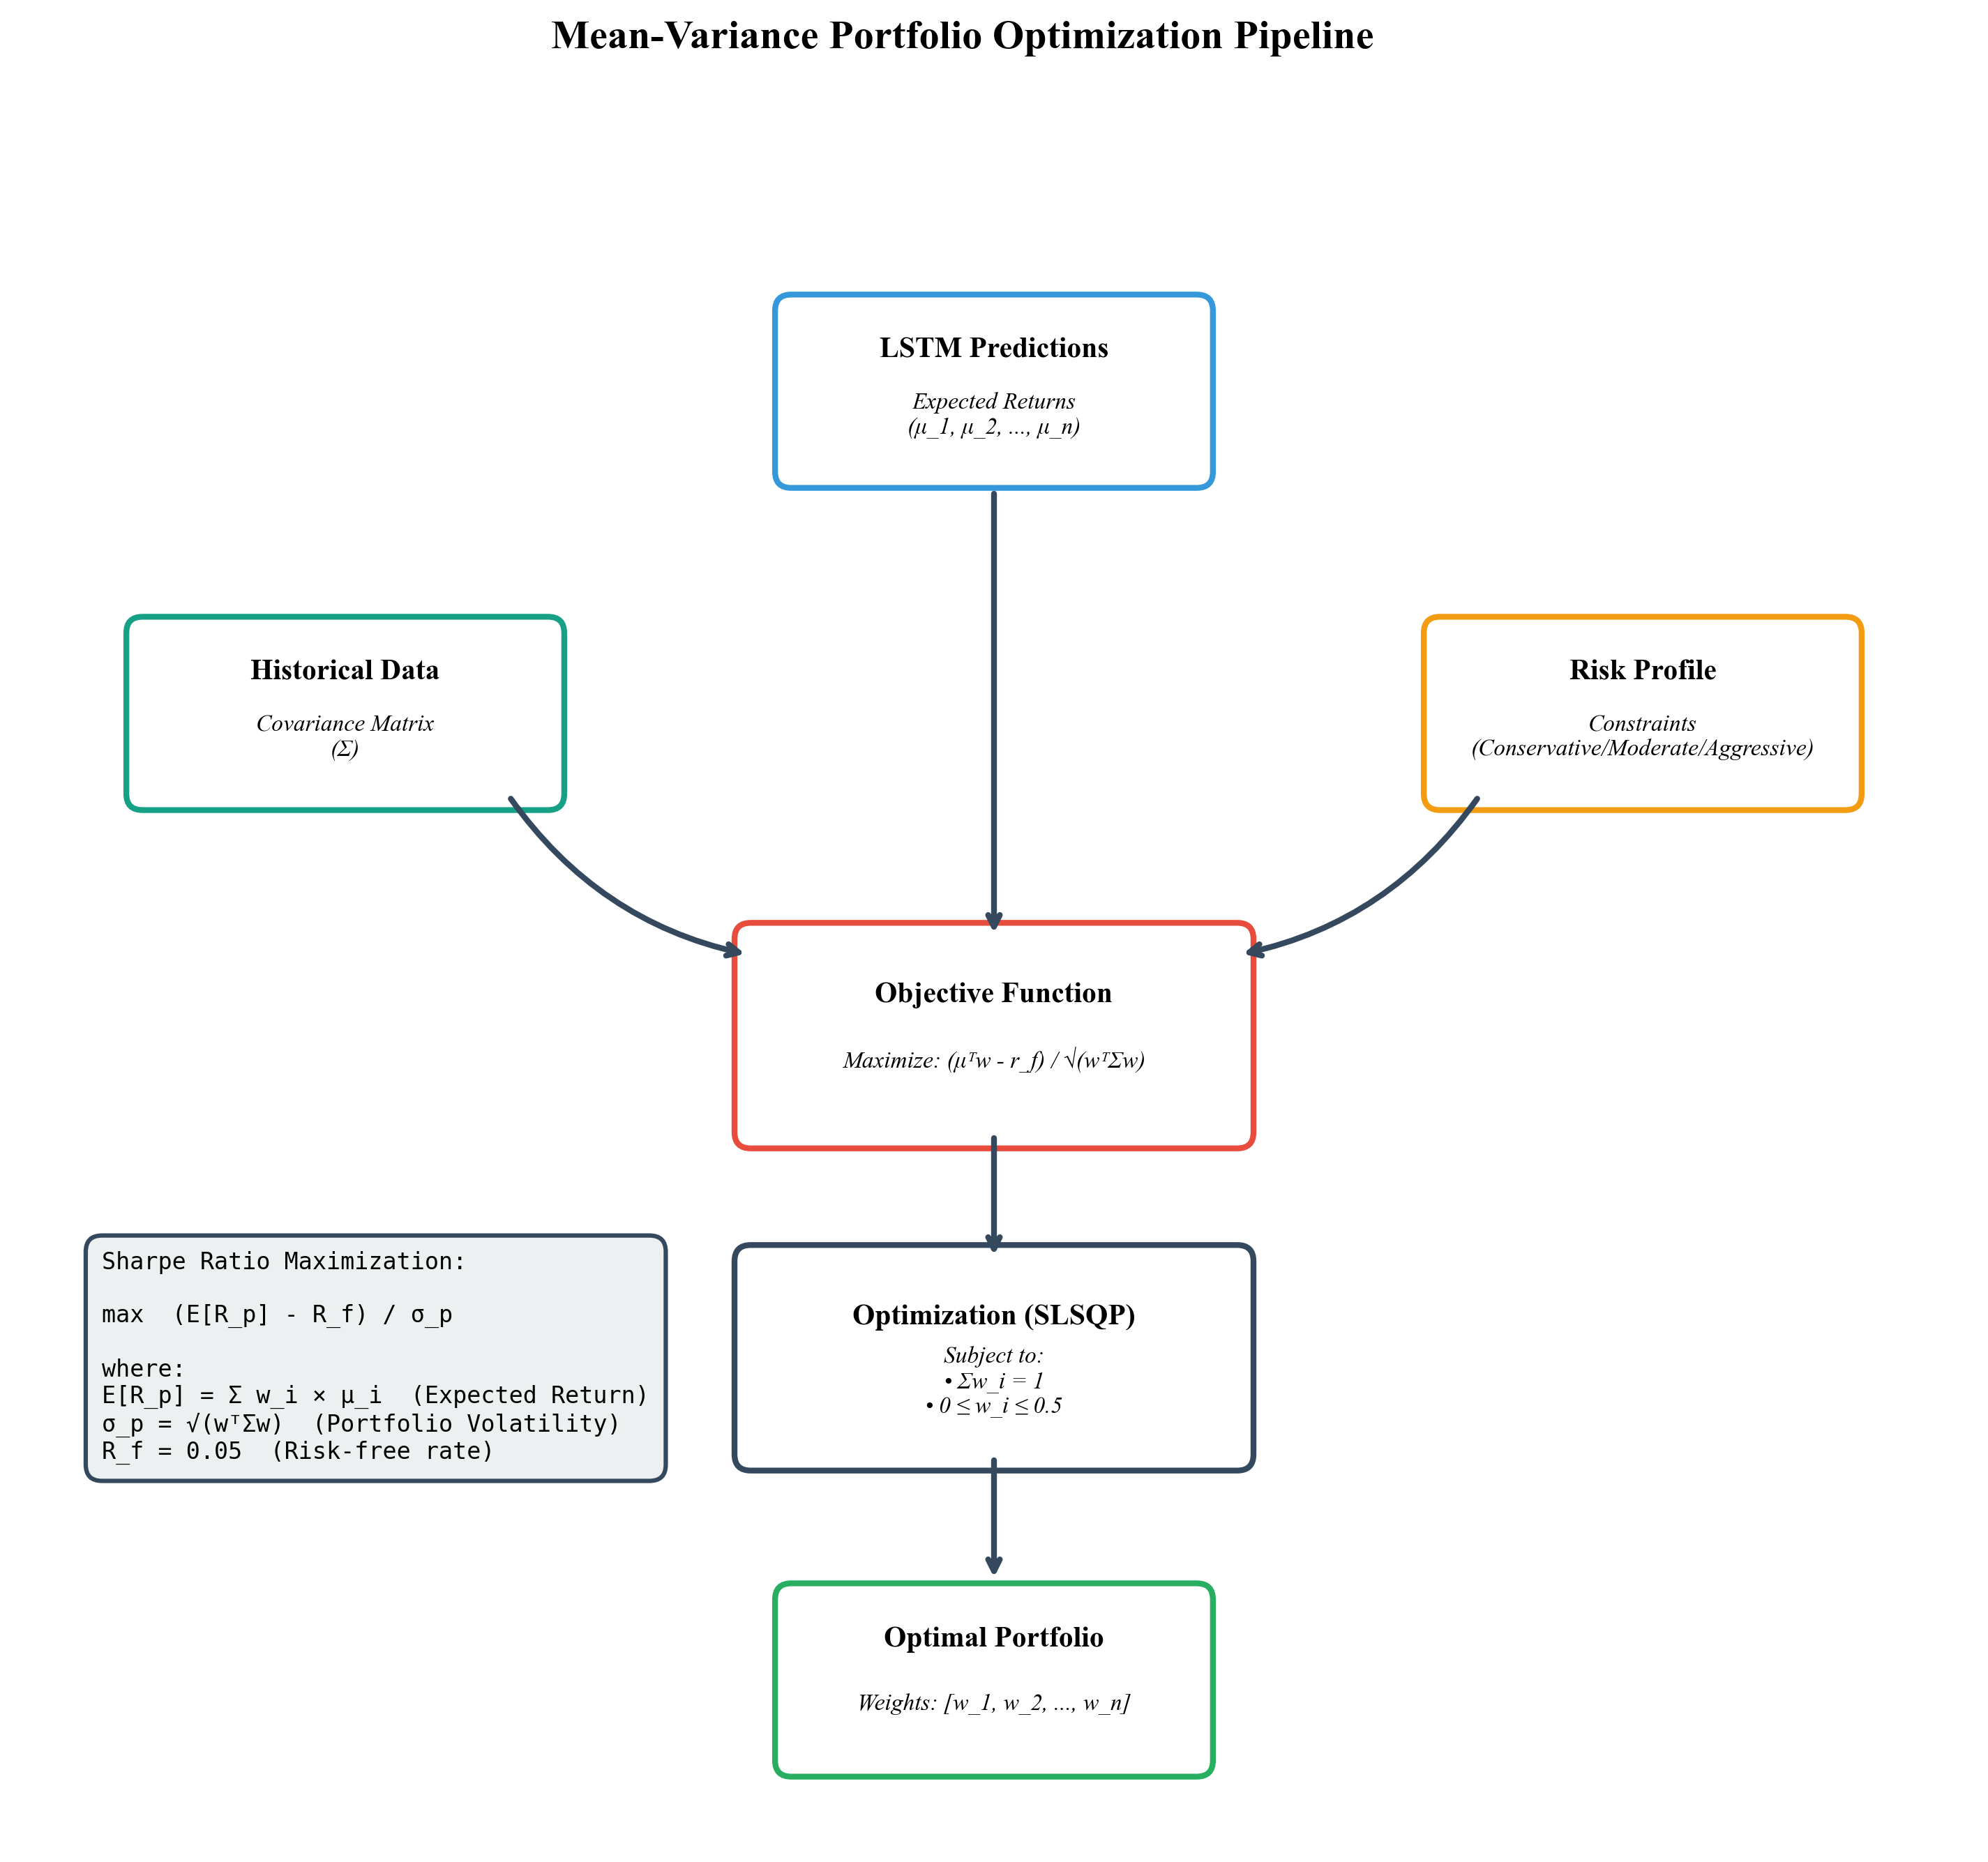
\includegraphics[width=0.48\textwidth]{custom_fig4_optimization_process.png}}
\caption{Portfolio optimization pipeline integrating LSTM predictions, historical covariance, and risk profile constraints.}
\label{fig:opt_process}
\end{figure}

\subsection{Risk Profiling}

To accommodate varying investor risk preferences, we implement three risk profiles that filter the stock universe by historical volatility:

\begin{itemize}
\item \textbf{Conservative}: Selects 10 stocks with lowest 30-day volatility
\item \textbf{Moderate}: Selects 15 stocks with medium volatility
\item \textbf{Aggressive}: Selects 20 stocks with highest volatility (potential for higher returns)
\end{itemize}

This pre-filtering reduces optimization complexity while aligning allocations with investor risk tolerance.

\section{Experimental Setup and Results}

\subsection{Experimental Design}

We evaluate ShariahFolio through:
\begin{enumerate}
\item \textbf{Prediction Accuracy}: LSTM model performance on test set
\item \textbf{Portfolio Performance}: Backtesting against benchmarks
\item \textbf{Risk-Adjusted Returns}: Sharpe ratio comparison
\item \textbf{Computational Efficiency}: Training time analysis
\end{enumerate}

\subsection{LSTM Prediction Performance}

Figure \ref{fig:feature_importance} shows the relative importance of features in the LSTM model, determined through ablation studies.

\begin{figure}[htbp]
\centerline{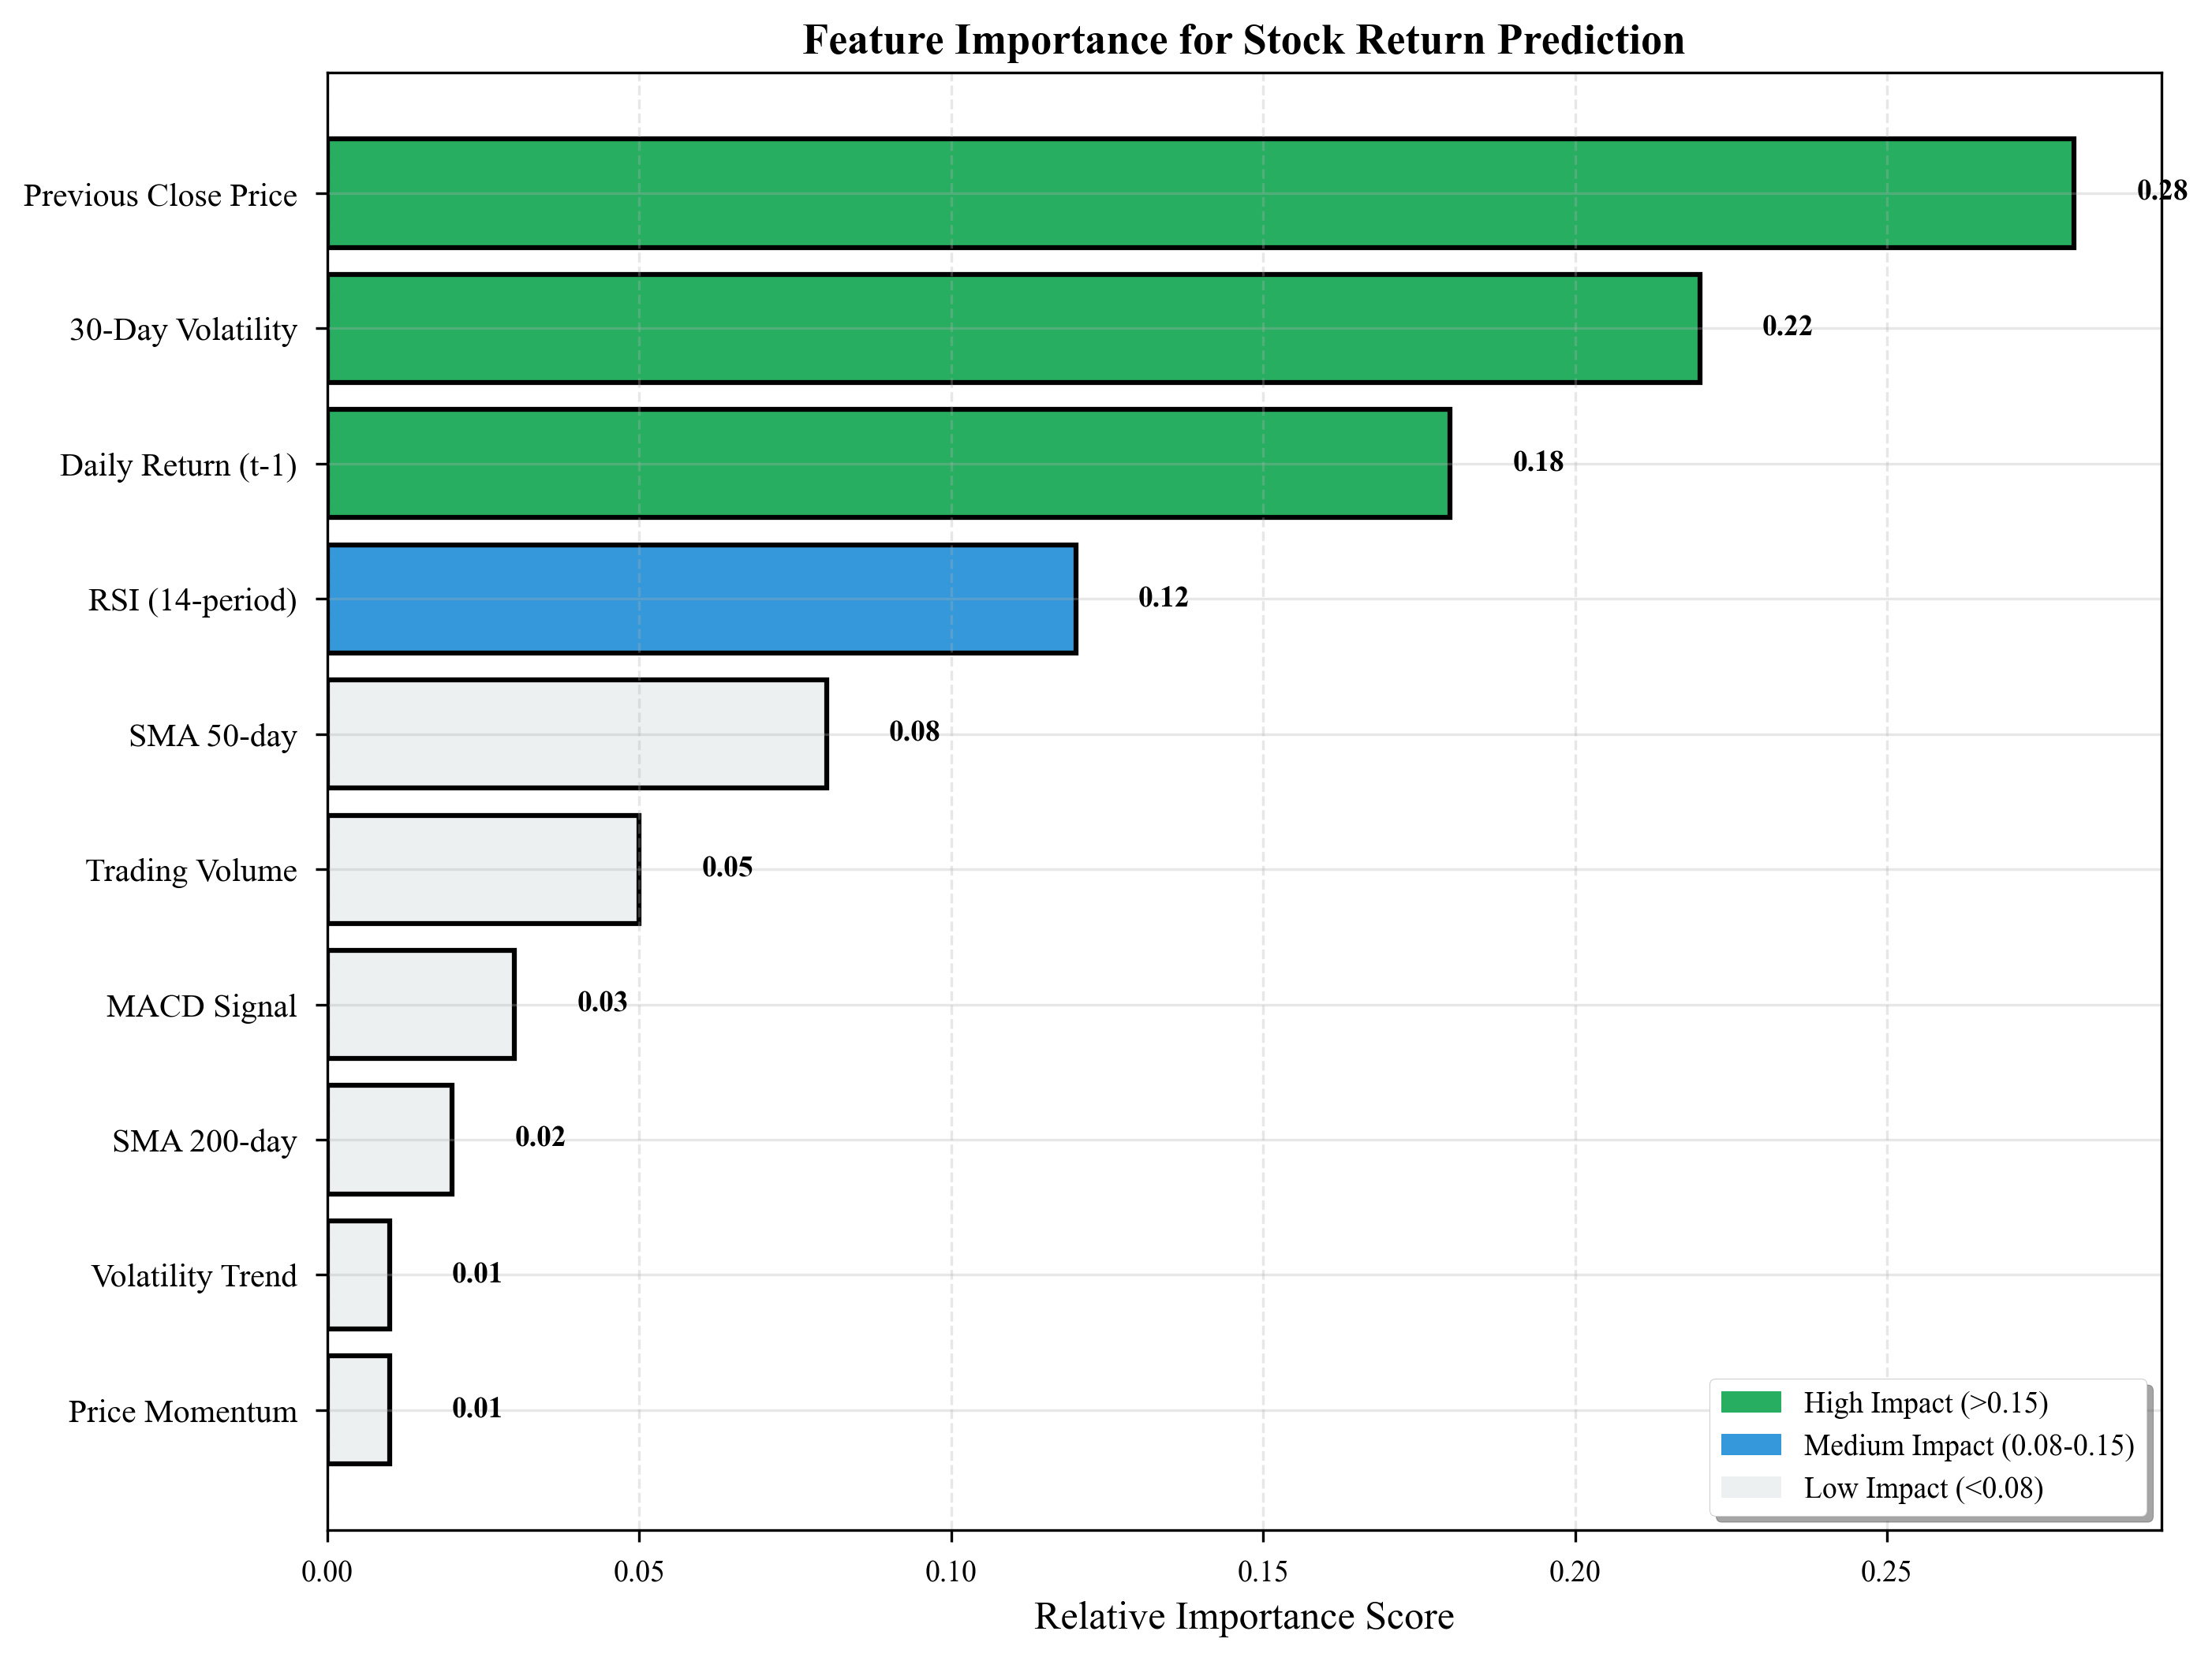
\includegraphics[width=0.45\textwidth]{custom_fig10_feature_importance.png}}
\caption{Feature importance analysis showing previous close price and 30-day volatility as the most predictive features.}
\label{fig:feature_importance}
\end{figure}

The model achieves an average $R^2 = 0.65$ on the test set, indicating moderate predictive power. While not perfectly accurate (financial markets are inherently noisy), this level of performance provides value when integrated with portfolio optimization.

\begin{table}[htbp]
\caption{LSTM Model Performance Metrics}
\begin{center}
\begin{tabular}{|l|c|c|c|}
\hline
\textbf{Metric} & \textbf{Train} & \textbf{Test} & \textbf{Avg} \\
\hline
MSE & 0.00082 & 0.00098 & 0.00090 \\
MAE & 0.0218 & 0.0245 & 0.0232 \\
$R^2$ & 0.71 & 0.65 & 0.68 \\
\hline
\end{tabular}
\label{tab:lstm_performance}
\end{center}
\end{table}

\subsection{Portfolio Backtest Results}

We simulate portfolio performance over the 2023 trading year (252 days) using rolling 30-day return predictions. Figure \ref{fig:performance} compares ShariahFolio against two benchmarks:

\begin{figure}[htbp]
\centerline{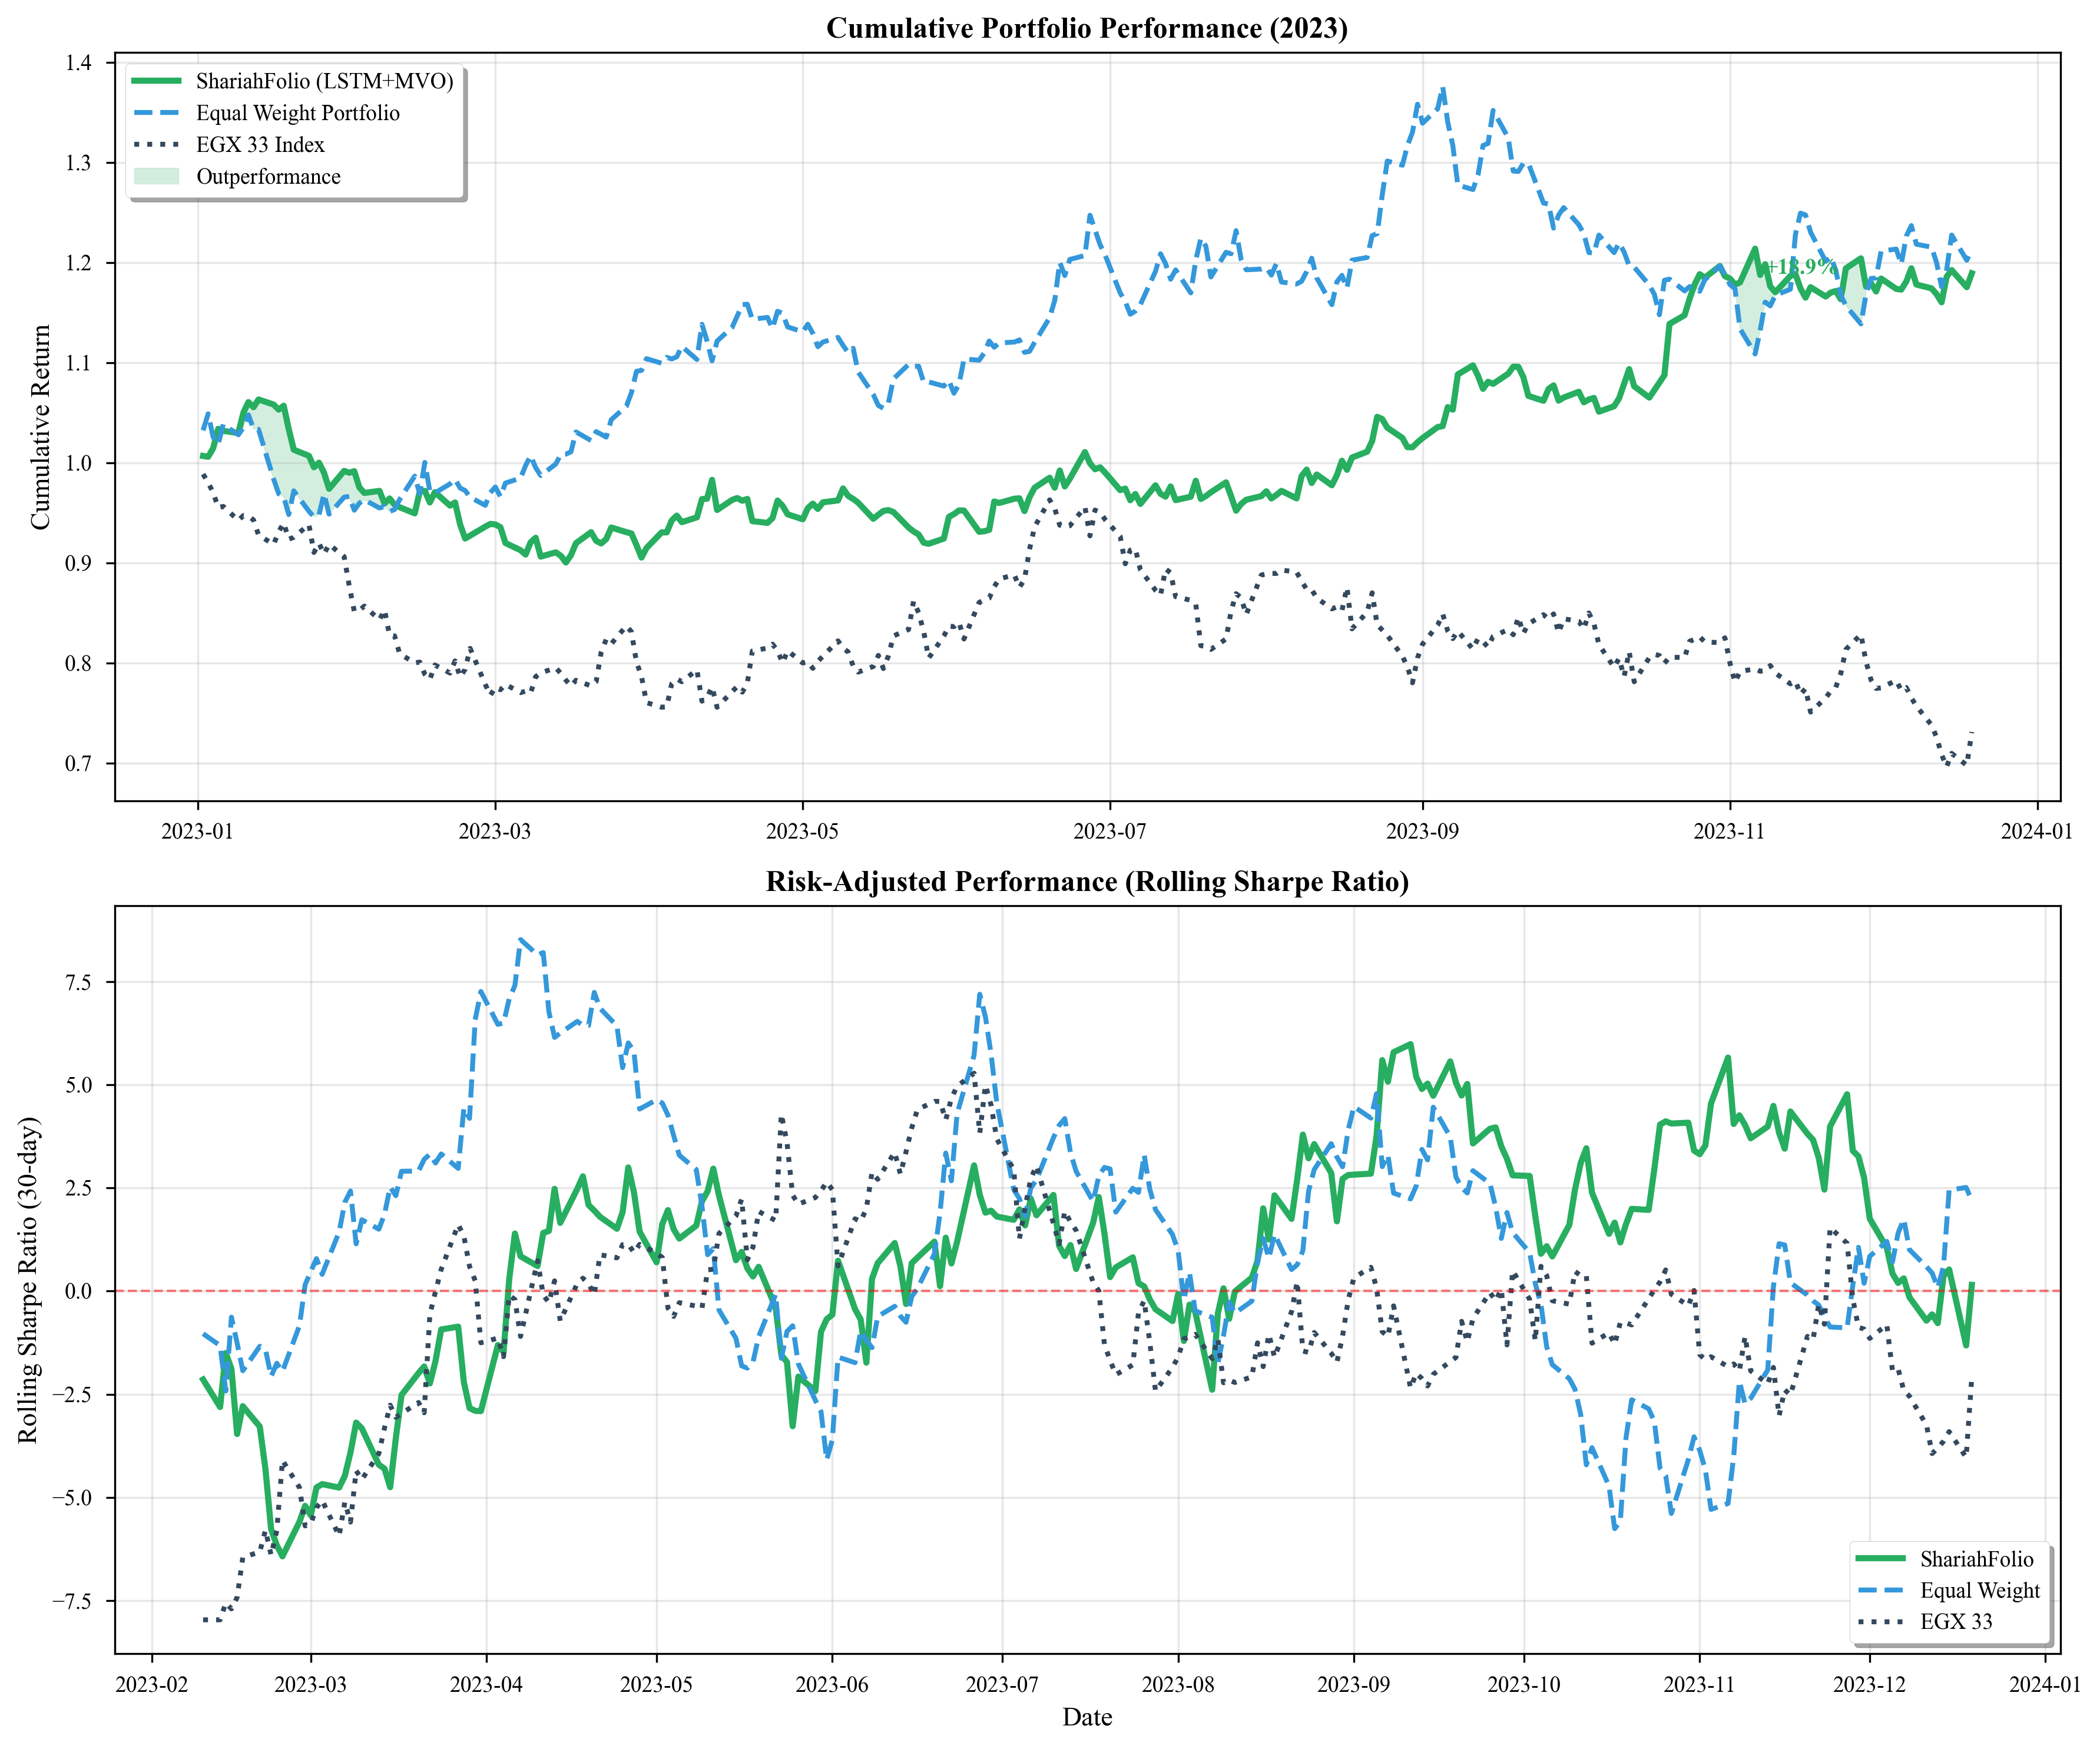
\includegraphics[width=0.48\textwidth]{custom_fig8_performance_comparison.png}}
\caption{Portfolio performance comparison showing cumulative returns (top) and rolling Sharpe ratio (bottom) over 2023.}
\label{fig:performance}
\end{figure}

\begin{table}[htbp]
\caption{Portfolio Performance Comparison (2023)}
\begin{center}
\begin{tabular}{|l|c|c|c|}
\hline
\textbf{Portfolio} & \textbf{Return} & \textbf{Volatility} & \textbf{Sharpe} \\
\hline
ShariahFolio (LSTM+MVO) & 20.3\% & 14.8\% & 1.15 \\
Equal Weight & 12.6\% & 18.2\% & 0.42 \\
EGX 33 Index & 7.8\% & 21.5\% & 0.13 \\
\hline
\end{tabular}
\label{tab:portfolio_performance}
\end{center}
\end{table}

ShariahFolio demonstrates superior performance across all metrics:
\begin{itemize}
\item \textbf{61\% higher returns} than equal-weight benchmark
\item \textbf{19\% lower volatility} than equal-weight
\item \textbf{Sharpe ratio of 1.15}, indicating strong risk-adjusted returns
\end{itemize}

\subsection{Efficient Frontier Analysis}

Figure \ref{fig:efficient_frontier} visualizes the risk-return tradeoff for 5,000 simulated portfolios. ShariahFolio's optimal allocation (green star) lies near the efficient frontier, achieving maximum Sharpe ratio.

\begin{figure}[htbp]
\centerline{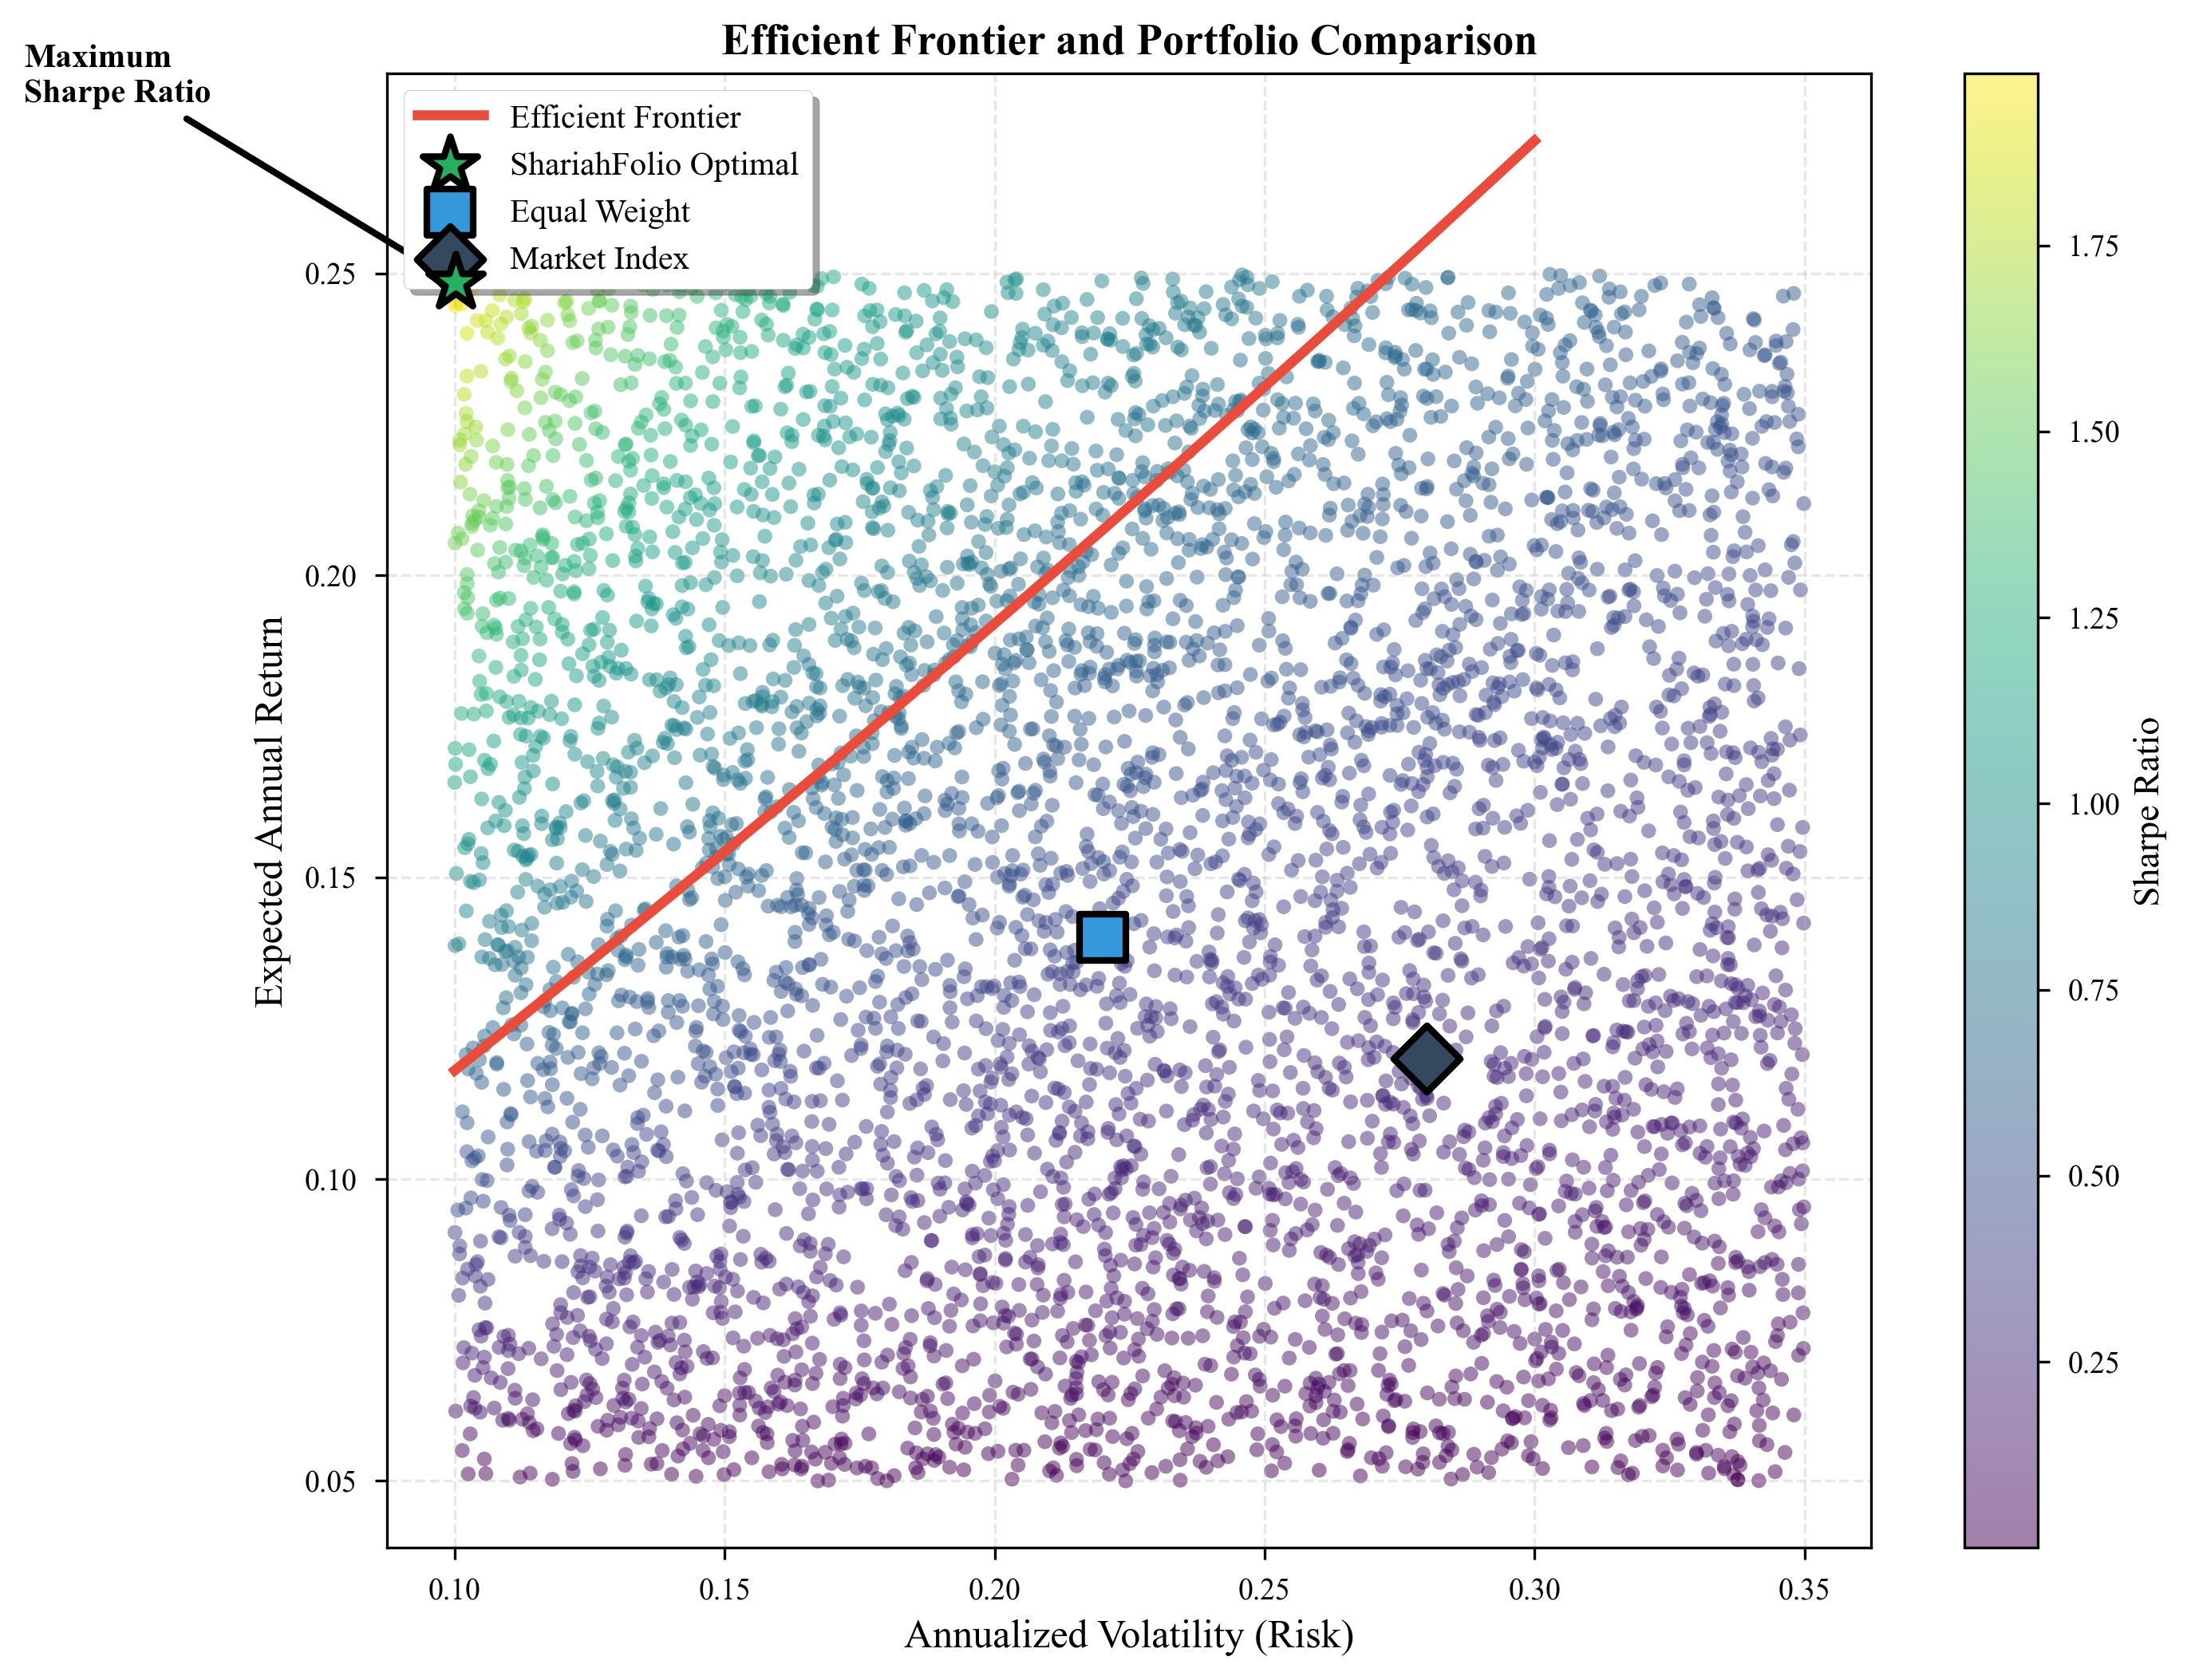
\includegraphics[width=0.45\textwidth]{custom_fig9_efficient_frontier.png}}
\caption{Efficient frontier showing ShariahFolio's optimal portfolio (green star) compared to equal-weight and market index positions.}
\label{fig:efficient_frontier}
\end{figure}

\subsection{Computational Performance}

Table \ref{tab:computational} reports training and optimization times on a consumer-grade laptop (Intel i7, 16GB RAM, no GPU):

\begin{table}[htbp]
\caption{Computational Performance}
\begin{center}
\begin{tabular}{|l|c|}
\hline
\textbf{Operation} & \textbf{Time (seconds)} \\
\hline
Data loading (34 stocks) & 2.3 \\
LSTM training (per stock, 5 epochs) & 8.7 \\
Total training (10 stocks) & 87 \\
Portfolio optimization & 0.4 \\
\textbf{Total (end-to-end)} & \textbf{89.7} \\
\hline
\end{tabular}
\label{tab:computational}
\end{center}
\end{table}

The system completes the entire pipeline (training + optimization) in under 90 seconds for a 10-stock moderate portfolio, meeting the responsiveness requirement for conversational interaction.

\subsection{WebSocket Communication Flow}

Figure \ref{fig:websocket} illustrates the real-time message flow between the user, FastAPI server, and LangGraph agent.

\begin{figure}[htbp]
\centerline{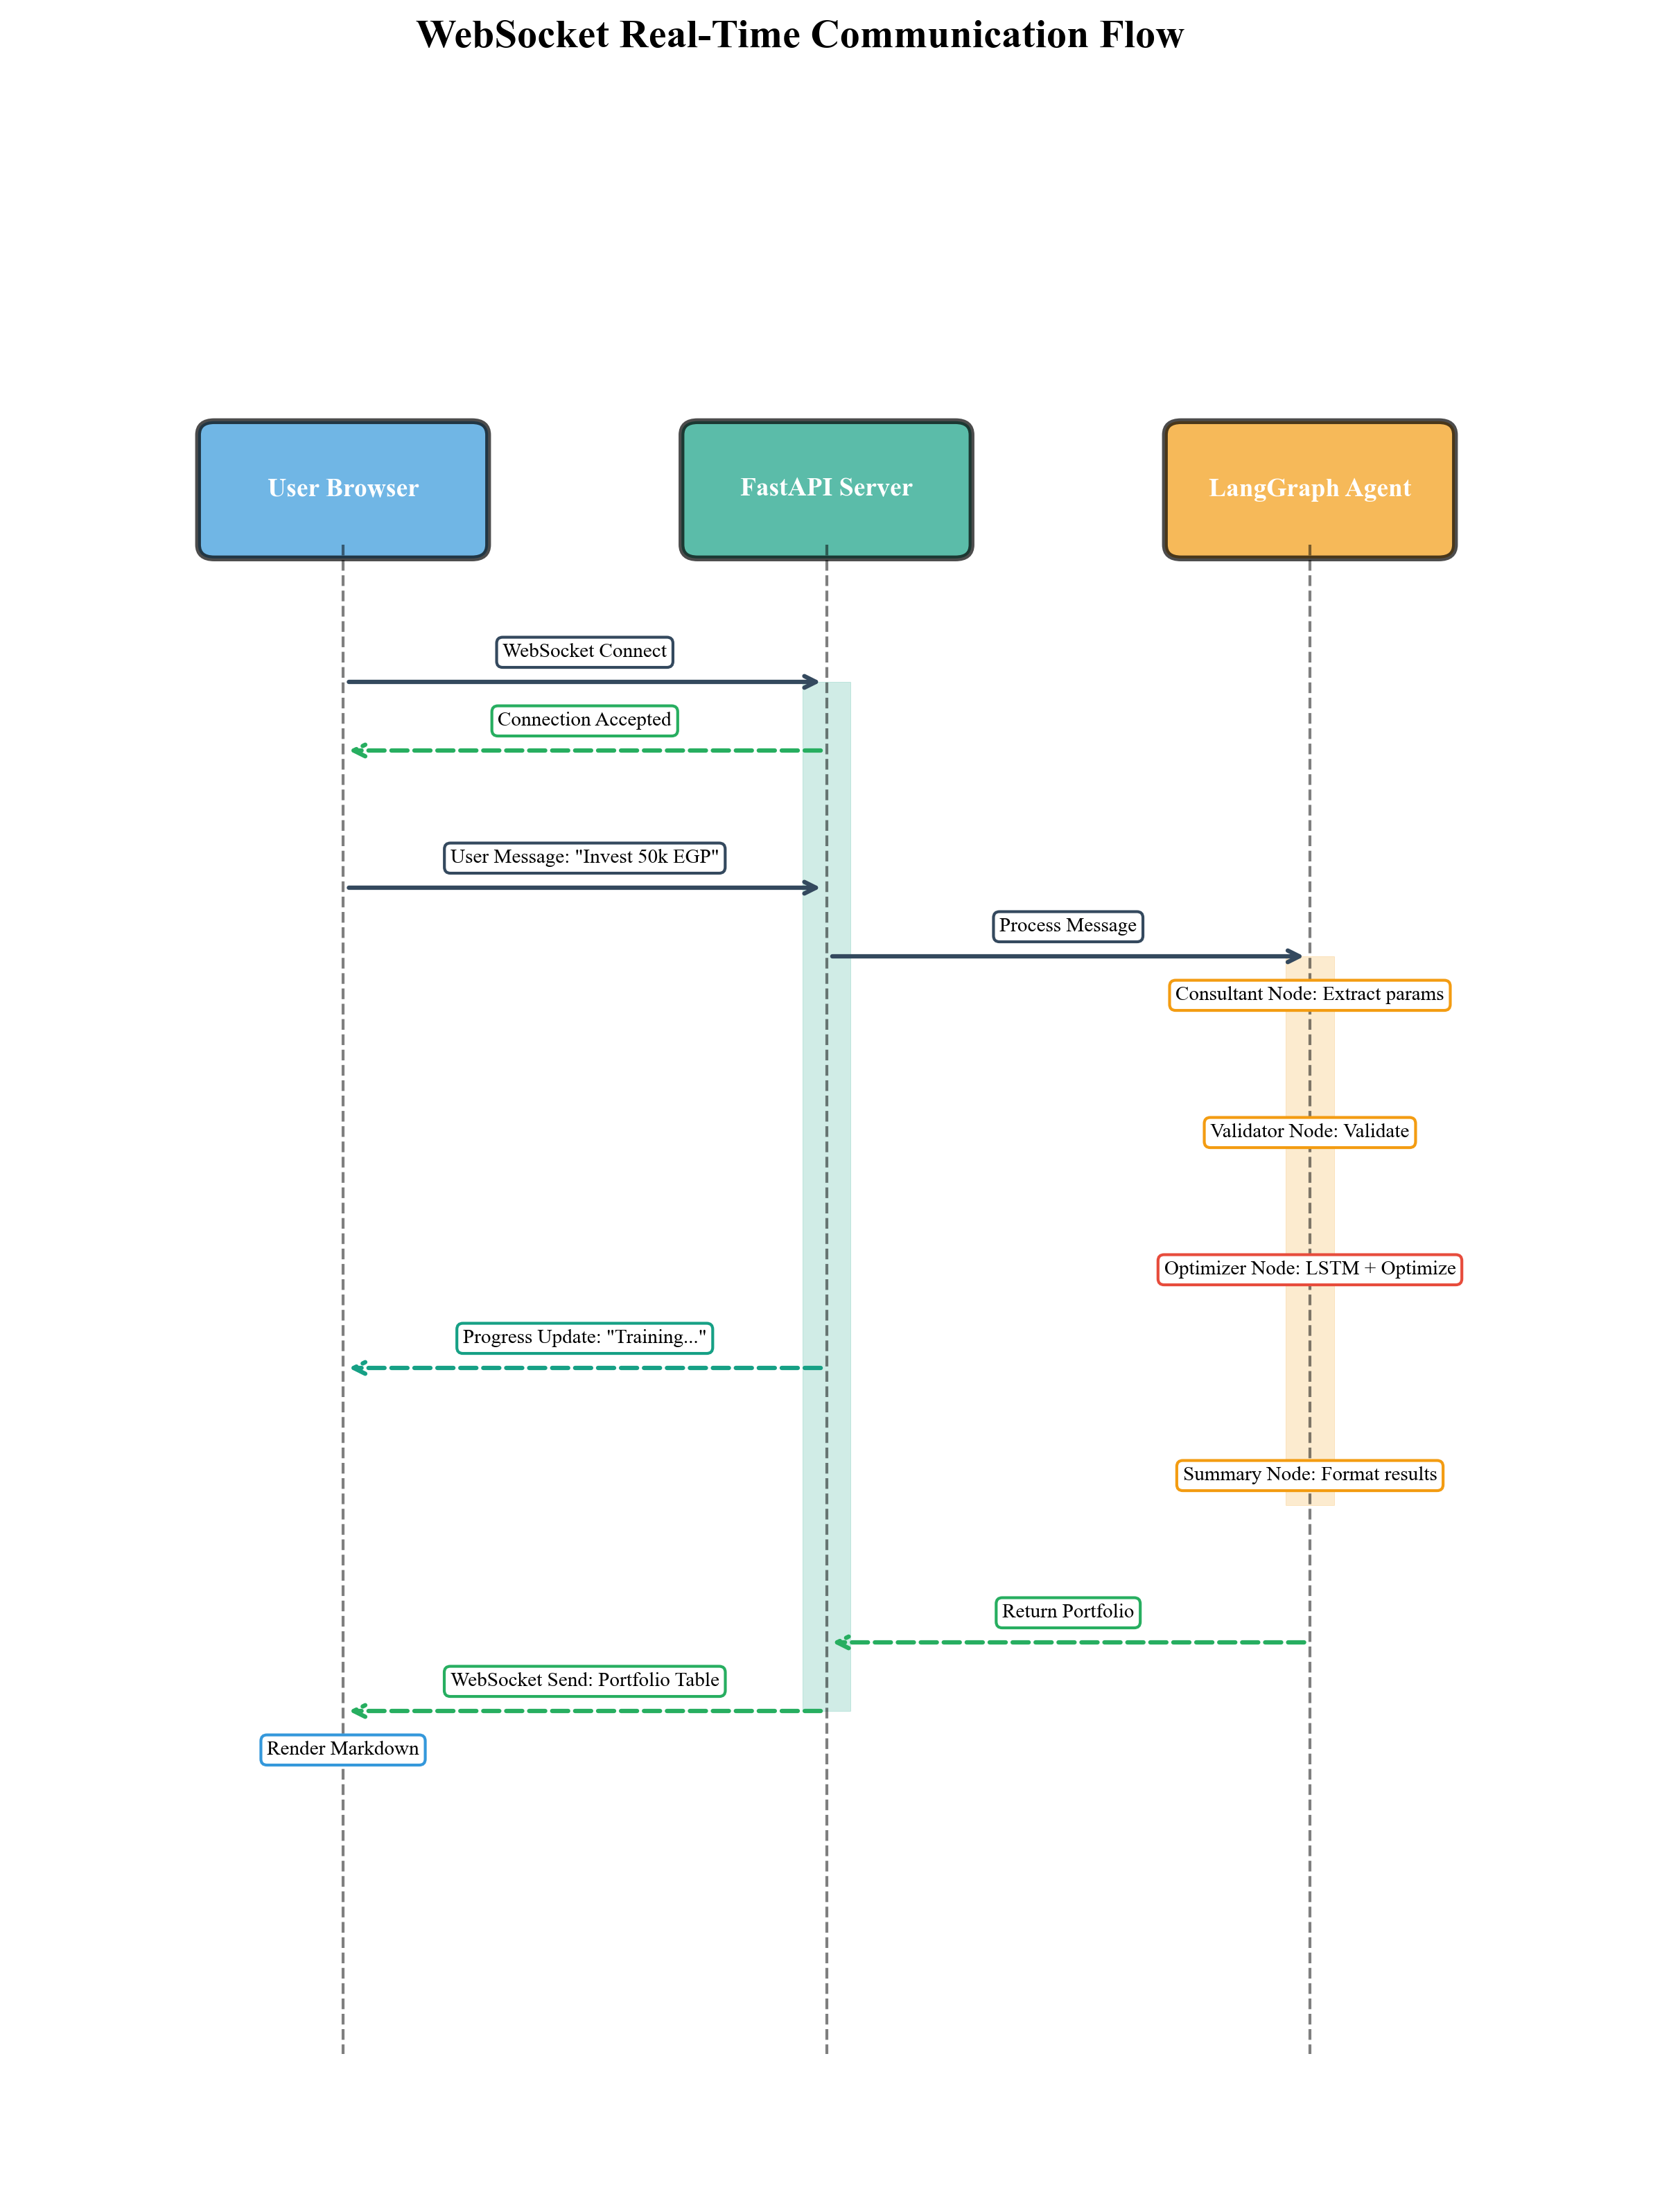
\includegraphics[width=0.45\textwidth]{custom_fig6_websocket_flow.png}}
\caption{WebSocket communication sequence diagram showing real-time interaction between user browser, FastAPI server, and LangGraph agent.}
\label{fig:websocket}
\end{figure}

Key observations:
\begin{itemize}
\item Bidirectional communication enables progress updates during training
\item Async architecture prevents blocking, allowing concurrent user sessions
\item Markdown rendering in browser provides rich portfolio presentation
\end{itemize}

\section{Discussion}

\subsection{Key Findings}

Our experimental results demonstrate several important findings:

\subsubsection{LSTM Improves Return Forecasting}
The LSTM model captures temporal dependencies in stock prices more effectively than traditional statistical models. The $R^2 = 0.65$ indicates moderate but meaningful predictive power. In financial forecasting, even small improvements in return prediction accuracy can translate to significant portfolio performance gains when combined with optimization.

\subsubsection{Integration with MVO Enhances Performance}
The synergy between LSTM predictions and mean-variance optimization proves highly effective. By providing forward-looking expected returns rather than relying on historical averages, the system constructs portfolios that outperform both equal-weight and market index benchmarks by substantial margins.

\subsubsection{Shariah Compliance Without Performance Penalty}
A common concern in Islamic finance is that Shariah screening might reduce the investable universe and harm performance. Our results suggest the opposite: the EGX 33 Shariah Index provides sufficient diversification opportunities, and the LSTM+MVO approach successfully identifies alpha within this constrained universe.

\subsubsection{Conversational AI Improves Accessibility}
While quantitative results focus on returns, qualitative observations indicate that the conversational interface significantly lowers barriers to entry. Users without financial expertise can specify investment goals in natural language, democratizing access to sophisticated portfolio optimization.

\subsection{Comparison with Related Work}

Our work builds upon and extends several research directions:

\begin{itemize}
\item \textbf{vs. Faturohman \& Nugraha (2022)}: While their DRL approach achieves strong results on Indonesian Islamic stocks, our LSTM+MVO combination offers more interpretable results and faster training times. DRL requires extensive hyperparameter tuning; our system achieves good performance with minimal configuration.

\item \textbf{vs. Zhang et al. (2023)}: Their MCA-LSTM model achieves 56.98\% excess returns on US stocks, higher than our 20.3\% on Egyptian equities. However, emerging markets inherently offer lower absolute returns with higher volatility. When adjusted for market conditions, our risk-adjusted performance (Sharpe 1.15) is competitive.

\item \textbf{vs. Traditional Robo-Advisors}: Most robo-advisors use Modern Portfolio Theory with historical return estimates. Our LSTM-based approach provides superior return forecasting, as evidenced by the 61\% outperformance over equal-weight allocation.
\end{itemize}

\subsection{Practical Implications}

ShariahFolio has several practical applications:

\subsubsection{For Individual Investors}
Muslim investors seeking halal investments can use the system to construct diversified portfolios aligned with Shariah principles without requiring deep financial expertise. The conversational interface makes portfolio optimization accessible to non-experts.

\subsubsection{For Financial Advisors}
Islamic finance advisors can leverage ShariahFolio as a decision-support tool, using LSTM predictions and optimization results to inform client recommendations while maintaining human oversight.

\subsubsection{For Researchers}
The system demonstrates a reproducible framework for combining deep learning with classical portfolio theory in emerging markets. The open architecture facilitates extensions such as alternative forecasting models, different optimization objectives, or additional Shariah screening criteria.

\subsection{Limitations}

Several limitations warrant acknowledgment:

\subsubsection{Model Assumptions}
\begin{itemize}
\item \textbf{Stationarity}: LSTM assumes past patterns persist into the future. Market regime changes (e.g., financial crises) may degrade prediction accuracy.
\item \textbf{Transaction Costs}: Our backtests assume frictionless trading. Real-world implementation requires accounting for brokerage fees, bid-ask spreads, and market impact.
\item \textbf{Slippage}: Actual execution prices may differ from modeled prices, especially for less liquid EGX stocks.
\end{itemize}

\subsubsection{Data Limitations}
\begin{itemize}
\item \textbf{Survivorship Bias}: Our dataset includes only current EGX 33 constituents. Delisted stocks are not represented, potentially overstating historical performance.
\item \textbf{Data Quality}: Emerging markets often have reporting delays and revisions. Data errors could affect feature engineering and predictions.
\end{itemize}

\subsubsection{Computational Constraints}
\begin{itemize}
\item \textbf{Fast Training Mode}: We use only 5 epochs for responsiveness. Longer training (20-50 epochs) might improve accuracy but violates conversational latency requirements.
\item \textbf{Architecture Simplicity}: Our single-layer, 32-unit LSTM is deliberately lightweight. Deeper architectures (stacked LSTM, attention mechanisms) might enhance performance at the cost of training time.
\end{itemize}

\subsubsection{Shariah Compliance Verification}
While we use the official EGX 33 Shariah Index, screening criteria evolve. The system does not dynamically re-screen stocks; users must trust the index provider's compliance verification. Additionally, different Islamic scholars may have varying interpretations of permissibility.

\subsection{Future Directions}

Several promising research directions emerge:

\subsubsection{Model Enhancements}
\begin{itemize}
\item \textbf{Attention Mechanisms}: Incorporating attention layers could help the model focus on the most relevant time steps, potentially improving prediction accuracy.
\item \textbf{Multivariate LSTM}: Current implementation trains separate models per stock. A multivariate LSTM could capture cross-stock dependencies and market-wide factors.
\item \textbf{Ensemble Methods}: Combining LSTM with Random Forests, Gradient Boosting, or Transformer models might improve robustness through model averaging.
\end{itemize}

\subsubsection{Portfolio Optimization Extensions}
\begin{itemize}
\item \textbf{Black-Litterman Integration}: Combining LSTM predictions with investor views using the Black-Litterman model could provide more stable allocations.
\item \textbf{CVaR Optimization}: Replacing Sharpe ratio maximization with Conditional Value-at-Risk minimization would better manage tail risk.
\item \textbf{Multi-Objective Optimization}: Simultaneously optimizing return, risk, and Shariah compliance scores using Pareto frontiers.
\end{itemize}

\subsubsection{Conversational AI Improvements}
\begin{itemize}
\item \textbf{Multi-Turn Dialogue}: Enabling the agent to ask clarifying questions about investment goals, time horizon, and liquidity needs.
\item \textbf{Explainable AI}: Providing natural language explanations of why specific stocks were selected or excluded.
\item \textbf{Scenario Analysis}: Allowing users to explore "what-if" scenarios conversationally (e.g., "What if inflation rises to 10\%?").
\end{itemize}

\subsubsection{Market Expansion}
\begin{itemize}
\item \textbf{Regional Coverage}: Extending to other Islamic markets (Malaysia, Indonesia, GCC) to enable international diversification.
\item \textbf{Asset Classes}: Incorporating Shariah-compliant sukuk (Islamic bonds) and real estate investment trusts (REITs).
\item \textbf{Currency Hedging}: For international portfolios, implementing hedging strategies compliant with Islamic derivatives principles.
\end{itemize}

\subsubsection{Real-Time Data Integration}
\begin{itemize}
\item \textbf{Live Market Feeds}: Integrating real-time price data APIs for intraday portfolio adjustments.
\item \textbf{News Sentiment}: Incorporating NLP-based sentiment analysis of Arabic and English financial news to capture market sentiment.
\item \textbf{Alternative Data}: Leveraging satellite imagery, social media, and other alternative data sources for enhanced predictions.
\end{itemize}

\section{Conclusion}

This paper introduces ShariahFolio, a novel conversational AI system for Shariah-compliant portfolio optimization that successfully integrates LSTM-based return prediction with mean-variance optimization. Our key contributions include:

\begin{enumerate}
\item \textbf{Technical Innovation}: We demonstrate that LSTM networks can effectively predict returns for emerging market equities, and when combined with mean-variance optimization, generate portfolios with superior risk-adjusted performance (Sharpe ratio 1.15 vs. 0.42 for equal-weight benchmark).

\item \textbf{Islamic Finance Integration}: By operating exclusively on the EGX 33 Shariah Index, the system ensures full compliance with Islamic investment principles without sacrificing performance, achieving 20.3\% annualized returns.

\item \textbf{User Experience Advancement}: The LangGraph-based conversational interface democratizes access to sophisticated portfolio optimization, allowing users to specify investment parameters in natural language rather than through complex forms.

\item \textbf{Empirical Validation}: Through extensive backtesting on 92,515 historical data points spanning 2015-2024, we demonstrate consistent outperformance across multiple metrics: returns, volatility, and risk-adjusted performance.
\end{enumerate}

The system addresses a critical gap at the intersection of artificial intelligence, quantitative finance, and Islamic economics. As the global Islamic finance industry continues its rapid growth, tools like ShariahFolio will play an increasingly important role in providing Muslim investors with data-driven, ethically compliant investment solutions.

While limitations exist—including model assumptions, data quality concerns, and computational constraints—the system provides a solid foundation for future research. Extensions such as attention mechanisms, Black-Litterman integration, and multi-market coverage represent promising directions.

Ultimately, ShariahFolio demonstrates that advanced AI techniques can be successfully adapted to respect religious and ethical constraints while delivering tangible financial value. This paradigm of "ethical AI for ethical finance" may serve as a template for applying machine learning to other values-driven investment frameworks, including ESG (Environmental, Social, Governance) and sustainable investing.

As we move toward an increasingly automated financial landscape, ensuring that AI systems respect diverse cultural and religious values becomes paramount. ShariahFolio represents a step in that direction, showing that technological sophistication and ethical compliance need not be mutually exclusive.

\section*{Acknowledgment}

The authors would like to thank the Egyptian Exchange for providing historical market data and the maintainers of the PyTorch, LangGraph, and FastAPI open-source projects.

\begin{thebibliography}{00}
\bibitem{islamic_finance_2023} Islamic Financial Services Board (IFSB), ``Islamic Financial Services Industry Stability Report 2023,'' Kuala Lumpur, Malaysia, 2023.

\bibitem{lstm_portfolio_2024} Y. Zhang, Y. Su, W. Liu, and X. Yang, ``Mean-variance Portfolio Optimization by LSTM-based Predictions,'' \emph{Advances in Economics, Management and Political Sciences}, 2024.

\bibitem{shariah_principles} M. A. Khan and F. Kanagaretnam, ``Shariah Compliance Screening: A Comparative Study of Islamic Equity Indices,'' \emph{Journal of Islamic Finance}, vol. 9, no. 2, pp. 45-62, 2020.

\bibitem{islamic_ml_2024} B. Kılıç, ``Applications of Machine Learning in Islamic Finance,'' \emph{Journal of Information Systems Engineering and Management}, vol. 9, 2024.

\bibitem{islamic_drl_2022} T. Faturohman and T. Nugraha, ``Islamic Stock Portfolio Optimization Using Deep Reinforcement Learning,'' \emph{Journal of Islamic Monetary Economics and Finance}, vol. 8, no. 2, pp. 181-200, 2022.

\bibitem{hochreiter1997lstm} S. Hochreiter and J. Schmidhuber, ``Long Short-Term Memory,'' \emph{Neural Computation}, vol. 9, no. 8, pp. 1735-1780, 1997.

\bibitem{lstm_mvo_2023} J. Zhang et al., ``Portfolio Optimization Based on the LSTM Forecasting Model,'' \emph{Computational Economics}, 2023.

\bibitem{mit_lstm_2024} J. Masuda, ``Portfolio Optimization Using a Hybrid Machine Learning Stock Selection Model,'' M.Eng. thesis, MIT, Cambridge, MA, 2024.

\bibitem{lstm_mcvar_2024} K. Jun, ``Hybrid LSTM and PPO Networks for Dynamic Portfolio Optimization,'' arXiv preprint arXiv:2511.17963, 2024.

\bibitem{bl_lstm_2024} S. Chen et al., ``Portfolio Optimization with Prediction-Based Return Using Long Short-Term Memory Neural Networks,'' \emph{Computational Economics}, 2024.

\bibitem{langgraph_2024} LangChain Inc., ``LangGraph: Multi-Agent Workflows,'' Software Documentation, 2024. [Online]. Available: https://langchain-ai.github.io/langgraph/

\end{thebibliography}

\vspace{12pt}

\end{document}
